\section{Capítulo IV - Desarrollo de la Metodología}
\label{cap:capitulo4}

\subsection{Formularios por Módulo}
\label{sec:cap4_formularios_modulo}

El presente capítulo documenta los formularios desarrollados para el Sistema Web de gestión contable, detallando la interfaz operativa, roles de acceso, endpoints de navegación, operaciones del ciclo de vida de datos (CRUD) y las validaciones críticas implementadas en el frontend (Angular) y backend (Python/FastAPI).

% =========================================================================
% MÓDULO 1: FACTURAS FEL/SAT
% =========================================================================
\subsubsection{Módulo: Facturas FEL/SAT}

{
\small
\setstretch{1.15}
\setlength{\parindent}{0pt}
\begin{xltabular}{\linewidth}{
    >{\raggedright\arraybackslash}p{1.3cm} 
    >{\raggedright\arraybackslash}p{2.2cm} 
    >{\raggedright\arraybackslash}>{\hsize=1.15\hsize}X 
    >{\raggedright\arraybackslash}>{\hsize=0.85\hsize}X 
    >{\centering\arraybackslash}p{0.6cm} 
    >{\raggedright\arraybackslash}p{2.0cm}
}

    % --- Encabezado de la primera página ---
    \caption{Resumen de formularios - Módulo: Facturas FEL/SAT} \label{tab:cap4_fel_resumen} \\
    \toprule
    \textbf{Código} & \textbf{Formulario} & \textbf{Propósito} & \textbf{Roles/Permisos} & \textbf{Op.} & \textbf{Ruta} \\
    \midrule
    \endfirsthead

    % --- Encabezado en páginas siguientes ---
    \toprule
    \textbf{Código} & \textbf{Formulario} & \textbf{Propósito} & \textbf{Roles/Permisos} & \textbf{Op.} & \textbf{Ruta} \\
    \midrule
    \endhead

    % --- Cierre en página intermedia ---
    \bottomrule
    \endfoot

    % --- Cierre final ---
    \bottomrule
    \endlastfoot

    % --- Filas de datos ---
    F-FEL-01 & Carga Masiva FEL & Importar archivos XML/Excel autorizados por la SAT & Admin, Auxiliar ({importar\_fel}) & C & {/facturas-fel} \\
    \addlinespace
    F-FEL-02 & Catálogo FEL & Consultar, filtrar y revisar facturas importadas & Admin, Contador, Auxiliar ({ver\_fel}) & R & {/facturas-fel} \\
    \addlinespace
    F-FEL-03 & Clasificación Contable & Asignar manualmente cuenta contable a factura no identificada & Admin, Contador ({clasificar\_fel}) & U & {/facturas-fel} \\
    \addlinespace
    F-FEL-04 & Anulación / Borrado & Marcar o retirar comprobante duplicado & Admin ({eliminar\_fel}) & D & {/facturas-fel} \\

\end{xltabular}
}

\paragraph{Formulario F-FEL-01: Carga Masiva y Procesamiento FEL}
\noindent\textbf{Objetivo:} Cargar e importar comprobantes tributarios electrónicos (XML o Excel) verificando la estructura del DTE y evitando la duplicidad de registros. \\[0.3em]
\textbf{Ubicación / Ruta:} Módulo Facturas FEL $\rightarrow$ Importación ({/facturas-fel}). \\[0.3em]
\textbf{Roles/Permisos:} Admin, Auxiliar ({importar\_fel}). \\[0.3em]
\textbf{Campos clave y validaciones críticas:} {archivo\_fel} (Requerido, formatos permitidos: {.xml}, {.xlsx}, tamaño máximo: 10 MB); {uuid\_dte} (Único, requerido - extraído automáticamente, formato UUID v4); {nit\_emisor} (Requerido, formato válido SAT, ej.: {1234567-8} o {CF}); {monto\_total} (Requerido, valor mayor a cero, $>0.00$). \\[0.3em]
\textbf{Flujo:} Arrastrar o seleccionar archivo $\rightarrow$ Análisis automático de estructura $\rightarrow$ Verificación de no duplicidad por UUID $\rightarrow$ Confirmación de carga $\rightarrow$ Actualización de catálogo. \\[0.3em]
\textbf{Mensaje principal del sistema:} ``Carga completada. Se procesaron $N$ facturas FEL exitosamente.''

\begin{figure}[H]
    \centering
    \caption{Módulo de Facturas FEL/SAT con opción de importación y catálogo.}
    \label{fig:cap4_fel_pantalla}
    \vspace{0.2cm}
    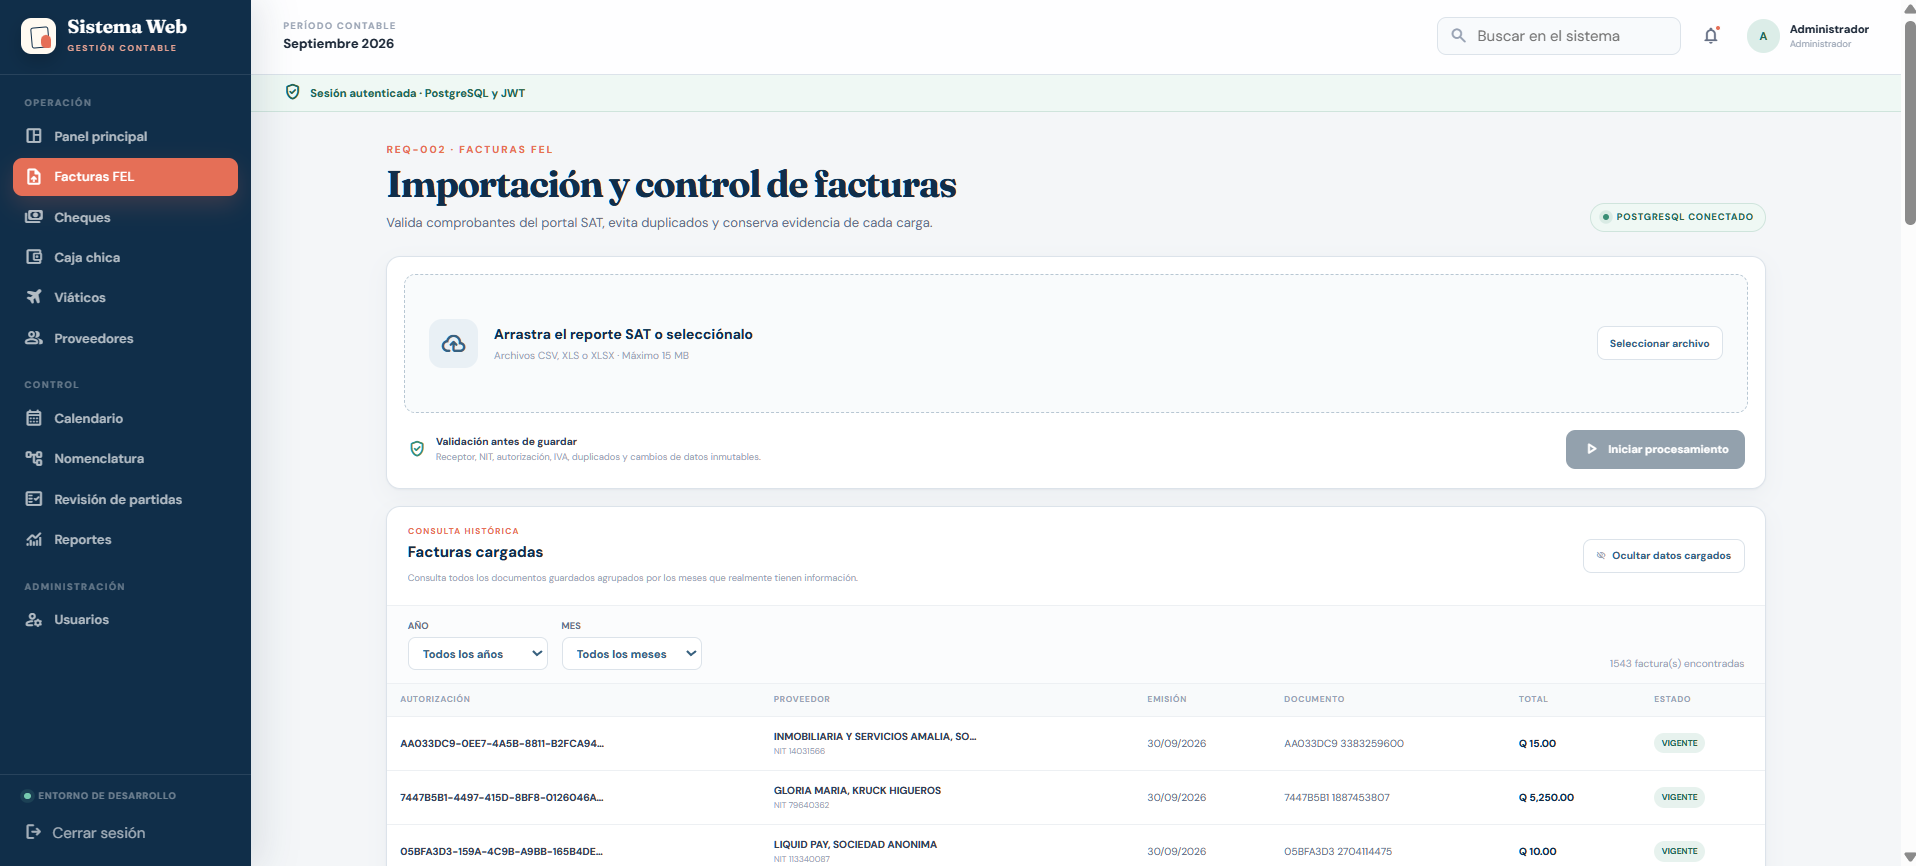
\includegraphics[width=0.96\linewidth]{capturas_reales/angular_actualizadas/pantalla_03_facturas_fel.png}
\end{figure}

% =========================================================================
% MÓDULO 2: CHEQUES POSFECHADOS
% =========================================================================
\subsubsection{Módulo: Cheques Posfechados}

{
\small
\setstretch{1.15}
\setlength{\parindent}{0pt}
\begin{xltabular}{\linewidth}{
    >{\raggedright\arraybackslash}p{1.3cm} 
    >{\raggedright\arraybackslash}p{2.2cm} 
    >{\raggedright\arraybackslash}>{\hsize=1.15\hsize}X 
    >{\raggedright\arraybackslash}>{\hsize=0.85\hsize}X 
    >{\centering\arraybackslash}p{0.6cm} 
    >{\raggedright\arraybackslash}p{2.0cm}
}

    % --- Encabezado de la primera página ---
    \caption{Resumen de formularios - Módulo: Cheques Posfechados} \label{tab:cap4_cheques_resumen} \\
    \toprule
    \textbf{Código} & \textbf{Formulario} & \textbf{Propósito} & \textbf{Roles/Permisos} & \textbf{Op.} & \textbf{Ruta} \\
    \midrule
    \endfirsthead

    % --- Encabezado en páginas siguientes ---
    \toprule
    \textbf{Código} & \textbf{Formulario} & \textbf{Propósito} & \textbf{Roles/Permisos} & \textbf{Op.} & \textbf{Ruta} \\
    \midrule
    \endhead

    % --- Cierre en página intermedia ---
    \bottomrule
    \endfoot

    % --- Cierre final ---
    \bottomrule
    \endlastfoot

    % --- Filas de datos ---
    F-CHEQ-01 & Control de Cheques & Registrar, consultar, actualizar estado y vincular a factura & Admin, Tesorero, Contador ({gestion\_cheques}) & CRUD & {/cheques} \\
    \addlinespace
    F-CHEQ-02 & Registro de Banco & Crear y administrar bancos emisores/receptores & Admin ({crear\_bancos}) & C & {/cheques} \\

\end{xltabular}
}

\paragraph{Formulario F-CHEQ-01: Gestión Integrada de Cheques Posfechados}
\noindent\textbf{Objetivo:} Registrar cheques de clientes, asociar banco receptor, dar seguimiento a fechas de depósito y vincular el pago a facturas emitidas. \\[0.3em]
\textbf{Ubicación / Ruta:} Módulo Cheques $\rightarrow$ Control de Cheques ({/cheques}). \\[0.3em]
\textbf{Roles/Permisos:} Admin, Tesorero, Contador ({gestion\_cheques}). \\[0.3em]
\textbf{Campos clave y validaciones críticas:} {numero\_cheque} (Requerido, numérico o alfanumérico único por banco, ej.: {CHQ-99482}); {cliente} (Requerido, texto o selección de catálogo); {banco\_origen} y {banco\_deposito} (Seleccionados de catálogo activo); {fecha\_recepcion} y {fecha\_deposito} (Requeridas, {fecha\_deposito} $\ge$ {fecha\_recepcion}); {monto} (Requerido, numérico mayor a cero, $>0.00$); {estado} (Requerido: Pendiente, Depositado, Rechazado). \\[0.3em]
\textbf{Flujo:} Hacer clic en ``Nuevo'' $\rightarrow$ Completar datos del cheque $\rightarrow$ Seleccionar factura o recibo en ``Asignación'' $\rightarrow$ Guardar registro. \\[0.3em]
\textbf{Mensaje principal del sistema:} ``Cheque registrado correctamente No. CHQ-99482.''

\begin{figure}[H]
    \centering
    \caption{Formulario y control de cheques posfechados anotado.}
    \label{fig:cap4_cheques_pantalla}
    \vspace{0.2cm}
    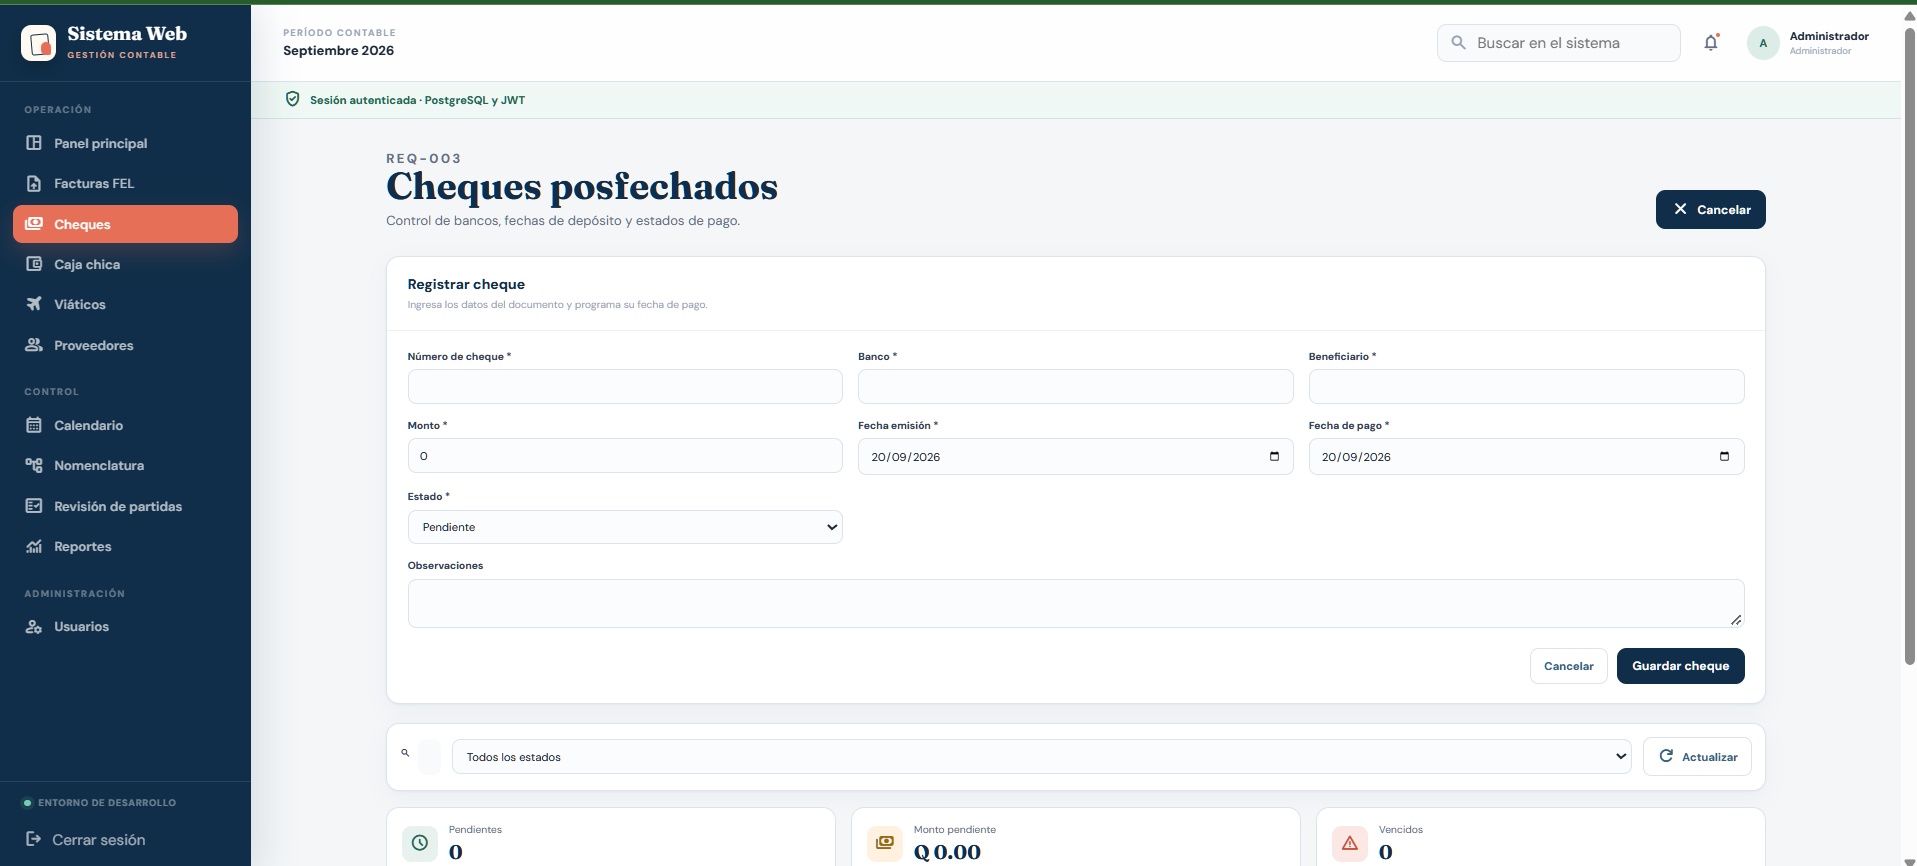
\includegraphics[width=0.96\linewidth]{capturas_reales/angular_actualizadas/formulario_cheque.png}
\end{figure}

% =========================================================================
% MÓDULO 3: CAJA CHICA
% =========================================================================
\subsubsection{Módulo: Caja Chica}

{
\small
\setstretch{1.15}
\setlength{\parindent}{0pt}
\begin{xltabular}{\linewidth}{
    >{\raggedright\arraybackslash}p{1.3cm} 
    >{\raggedright\arraybackslash}p{2.2cm} 
    >{\raggedright\arraybackslash}>{\hsize=1.15\hsize}X 
    >{\raggedright\arraybackslash}>{\hsize=0.85\hsize}X 
    >{\centering\arraybackslash}p{0.6cm} 
    >{\raggedright\arraybackslash}p{2.0cm}
}

    % --- Encabezado de la primera página ---
    \caption{Resumen de formularios - Módulo: Caja Chica} \label{tab:cap4_cajachica_resumen} \\
    \toprule
    \textbf{Código} & \textbf{Formulario} & \textbf{Propósito} & \textbf{Roles/Permisos} & \textbf{Op.} & \textbf{Ruta} \\
    \midrule
    \endfirsthead

    % --- Encabezado en páginas siguientes ---
    \toprule
    \textbf{Código} & \textbf{Formulario} & \textbf{Propósito} & \textbf{Roles/Permisos} & \textbf{Op.} & \textbf{Ruta} \\
    \midrule
    \endhead

    % --- Cierre en página intermedia ---
    \bottomrule
    \endfoot

    % --- Cierre final ---
    \bottomrule
    \endlastfoot

    % --- Filas de datos ---
    F-CAJA-01 & Asignar Factura FEL & Vincular factura FEL al fondo de Caja Chica & Admin, Operativo ({caja\_asigna\_fel}) & C & {/caja-chica} \\
    \addlinespace
    F-CAJA-02 & Nuevo Recibo & Registrar egreso de fondo sin comprobante FEL & Admin, Operativo ({caja\_recibos}) & C & {/caja-chica} \\
    \addlinespace
    F-CAJA-03 & Generación Partida & Crear asiento contable de liquidación y arqueo & Admin, Contador ({caja\_partidas}) & C/U & {/caja-chica} \\
    \addlinespace
    F-CAJA-04 & Resumen de Fondo & Visualización e impresión de arqueo del período & Admin, Contador, Auxiliar ({caja\_resumen}) & R & {/caja-chica} \\

\end{xltabular}
}

\paragraph{Formulario F-CAJA-02: Registro de Recibo / Egreso de Caja Chica}
\noindent\textbf{Objetivo:} Registrar egresos del fondo fijo respaldados por vales o recibos internos, sugiriendo o clasificando la cuenta contable de gasto. \\[0.3em]
\textbf{Ubicación / Ruta:} Módulo Caja Chica $\rightarrow$ Nuevo Recibo ({/caja-chica}). \\[0.3em]
\textbf{Roles/Permisos:} Admin, Operativo ({caja\_recibos}). \\[0.3em]
\textbf{Campos clave y validaciones críticas:} {fecha\_movimiento} (Requerida, dentro del período contable activo); {tipo\_documento} (Requerido: Recibo, Vale, Factura Exenta); {numero\_documento} (Requerido, ej.: {REC-00124}); {nombre\_beneficiario} (Requerido); {monto\_total} (Requerido, no puede exceder el fondo disponible, $>0.00$); {cuenta\_contable} (Requerida, seleccionada de Nomenclatura). \\[0.3em]
\textbf{Flujo:} Presionar ``Nuevo recibo'' $\rightarrow$ Capturar datos y monto $\rightarrow$ Asignar o validar cuenta contable de Nomenclatura $\rightarrow$ Guardar registro $\rightarrow$ Actualizar saldo del fondo. \\[0.3em]
\textbf{Mensaje principal del sistema:} ``Movimiento de Caja Chica registrado exitosamente.''

\begin{figure}[H]
    \centering
    \caption{Módulo de Caja Chica con captura de recibos y liquidación.}
    \label{fig:cap4_cajachica_pantalla}
    \vspace{0.2cm}
    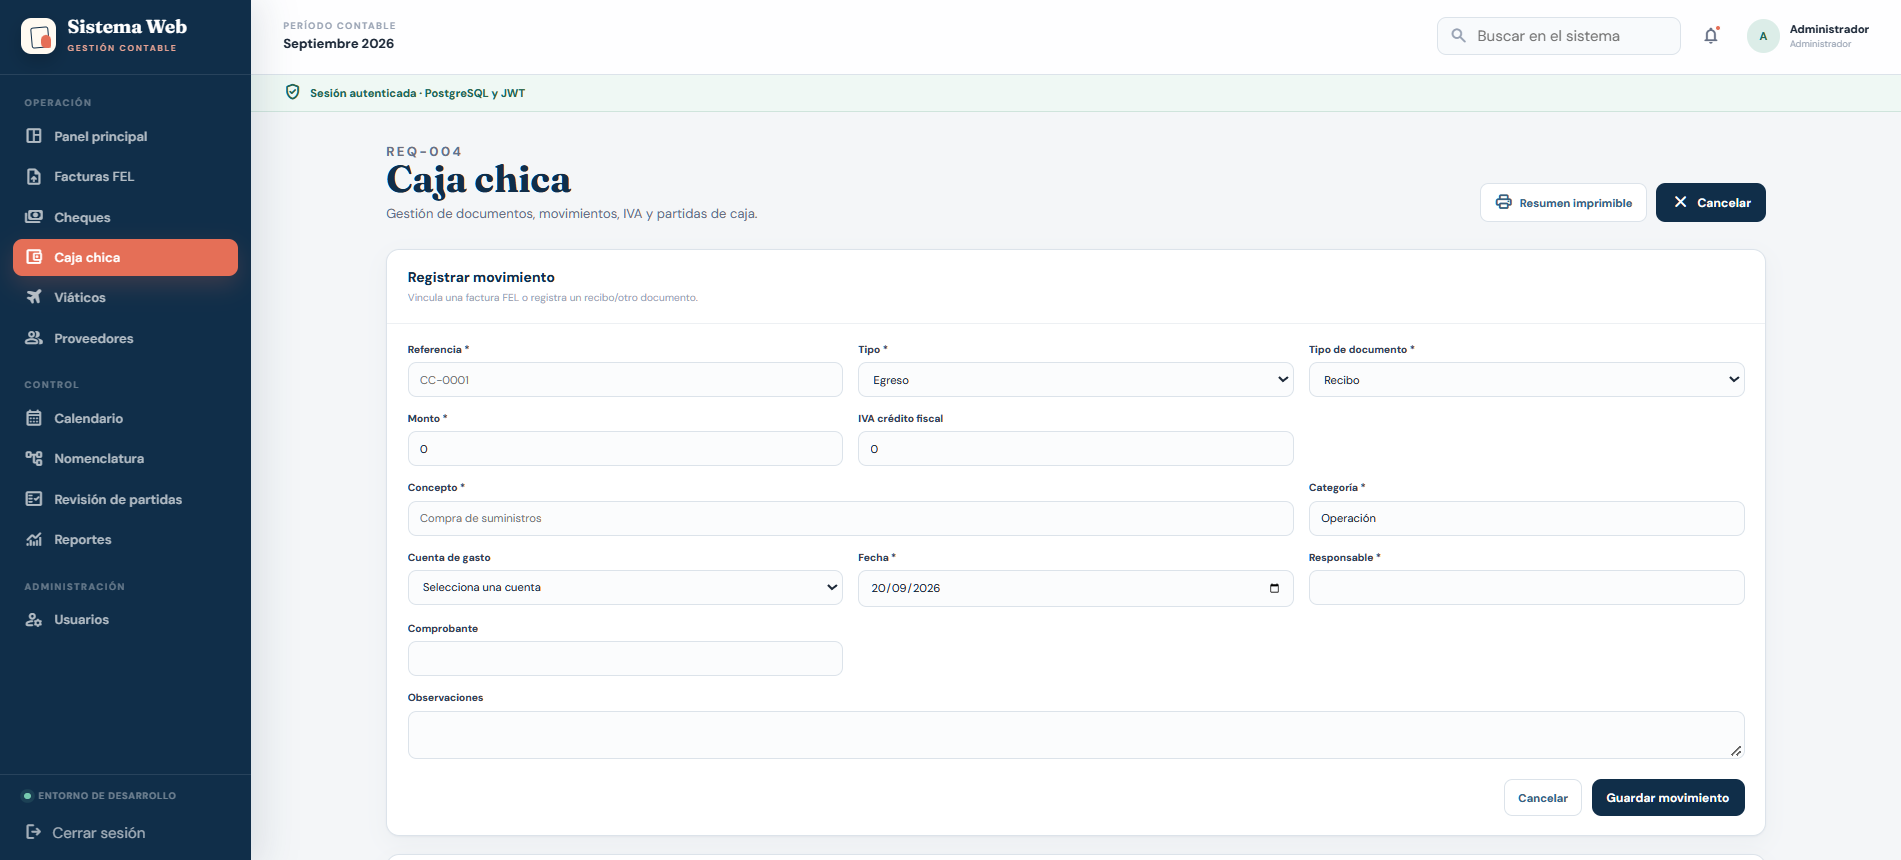
\includegraphics[width=0.96\linewidth]{capturas_reales/angular_actualizadas/formulario_caja_chica.png}
\end{figure}

% =========================================================================
% MÓDULO 4: VIÁTICOS
% =========================================================================
\subsubsection{Módulo: Viáticos}

{
\small
\setstretch{1.15}
\setlength{\parindent}{0pt}
\begin{xltabular}{\linewidth}{
    >{\raggedright\arraybackslash}p{1.3cm} 
    >{\raggedright\arraybackslash}p{2.2cm} 
    >{\raggedright\arraybackslash}>{\hsize=1.15\hsize}X 
    >{\raggedright\arraybackslash}>{\hsize=0.85\hsize}X 
    >{\centering\arraybackslash}p{0.6cm} 
    >{\raggedright\arraybackslash}p{2.0cm}
}

    % --- Encabezado de la primera página ---
    \caption{Resumen de formularios - Módulo: Viáticos} \label{tab:cap4_viaticos_resumen} \\
    \toprule
    \textbf{Código} & \textbf{Formulario} & \textbf{Propósito} & \textbf{Roles/Permisos} & \textbf{Op.} & \textbf{Ruta} \\
    \midrule
    \endfirsthead

    % --- Encabezado en páginas siguientes ---
    \toprule
    \textbf{Código} & \textbf{Formulario} & \textbf{Propósito} & \textbf{Roles/Permisos} & \textbf{Op.} & \textbf{Ruta} \\
    \midrule
    \endhead

    % --- Cierre en página intermedia ---
    \bottomrule
    \endfoot

    % --- Cierre final ---
    \bottomrule
    \endlastfoot

    % --- Filas de datos ---
    F-VIAT-01 & Gestión de Giras & Asignar territorio, colaborador y semana operativa & Admin, Encargado ({giras\_crear}) & C/U & {/viaticos} \\
    \addlinespace
    F-VIAT-02 & Asignación Factura & Vincular facturas FEL/recibos a categoría de viático & Admin, Encargado ({viaticos\_asigna}) & C & {/viaticos/asignacion} \\
    \addlinespace
    F-VIAT-03 & Generación Partida & Construir partida semanal o transitoria balanceada & Admin, Contador ({viaticos\_partida}) & C & {/viaticos} \\

\end{xltabular}
}

\paragraph{Formulario F-VIAT-02: Asignación de Facturas de Viáticos}
\noindent\textbf{Objetivo:} Asociar un comprobante de gasto a un colaborador, territorio, gira y categoría de viático (Viáticos, Movilidad o Actividades). \\[0.3em]
\textbf{Ubicación / Ruta:} Viáticos $\rightarrow$ Asignación de facturas ({/viaticos/asignacion}). \\[0.3em]
\textbf{Roles/Permisos:} Admin, Encargado ({viaticos\_asigna}). \\[0.3em]
\textbf{Campos clave y validaciones críticas:} {colaborador} (Seleccionado del catálogo de colaboradores activos); {territorio\_gira} (Requerido, debe coincidir con la semana programada); {categoria\_gasto} (Requerida: Viáticos, Movilidad, Actividades. Regla: Movilidad solo permitida la 1era semana del mes); {numero\_factura} (Requerido, no reutilizable en otra gira); {cuenta\_contable} (Requerida, seleccionada del catálogo de Nomenclatura). \\[0.3em]
\textbf{Flujo:} Seleccionar colaborador y gira $\rightarrow$ Ingresar número de factura $\rightarrow$ Asignar categoría y cuenta contable $\rightarrow$ Guardar asignación. \\[0.3em]
\textbf{Mensaje principal del sistema:} ``Factura asignada a gira correctamente.''

\begin{figure}[H]
    \centering
    \caption{Formulario de asignación de facturas a giras y viáticos.}
    \label{fig:cap4_viaticos_pantalla}
    \vspace{0.2cm}
    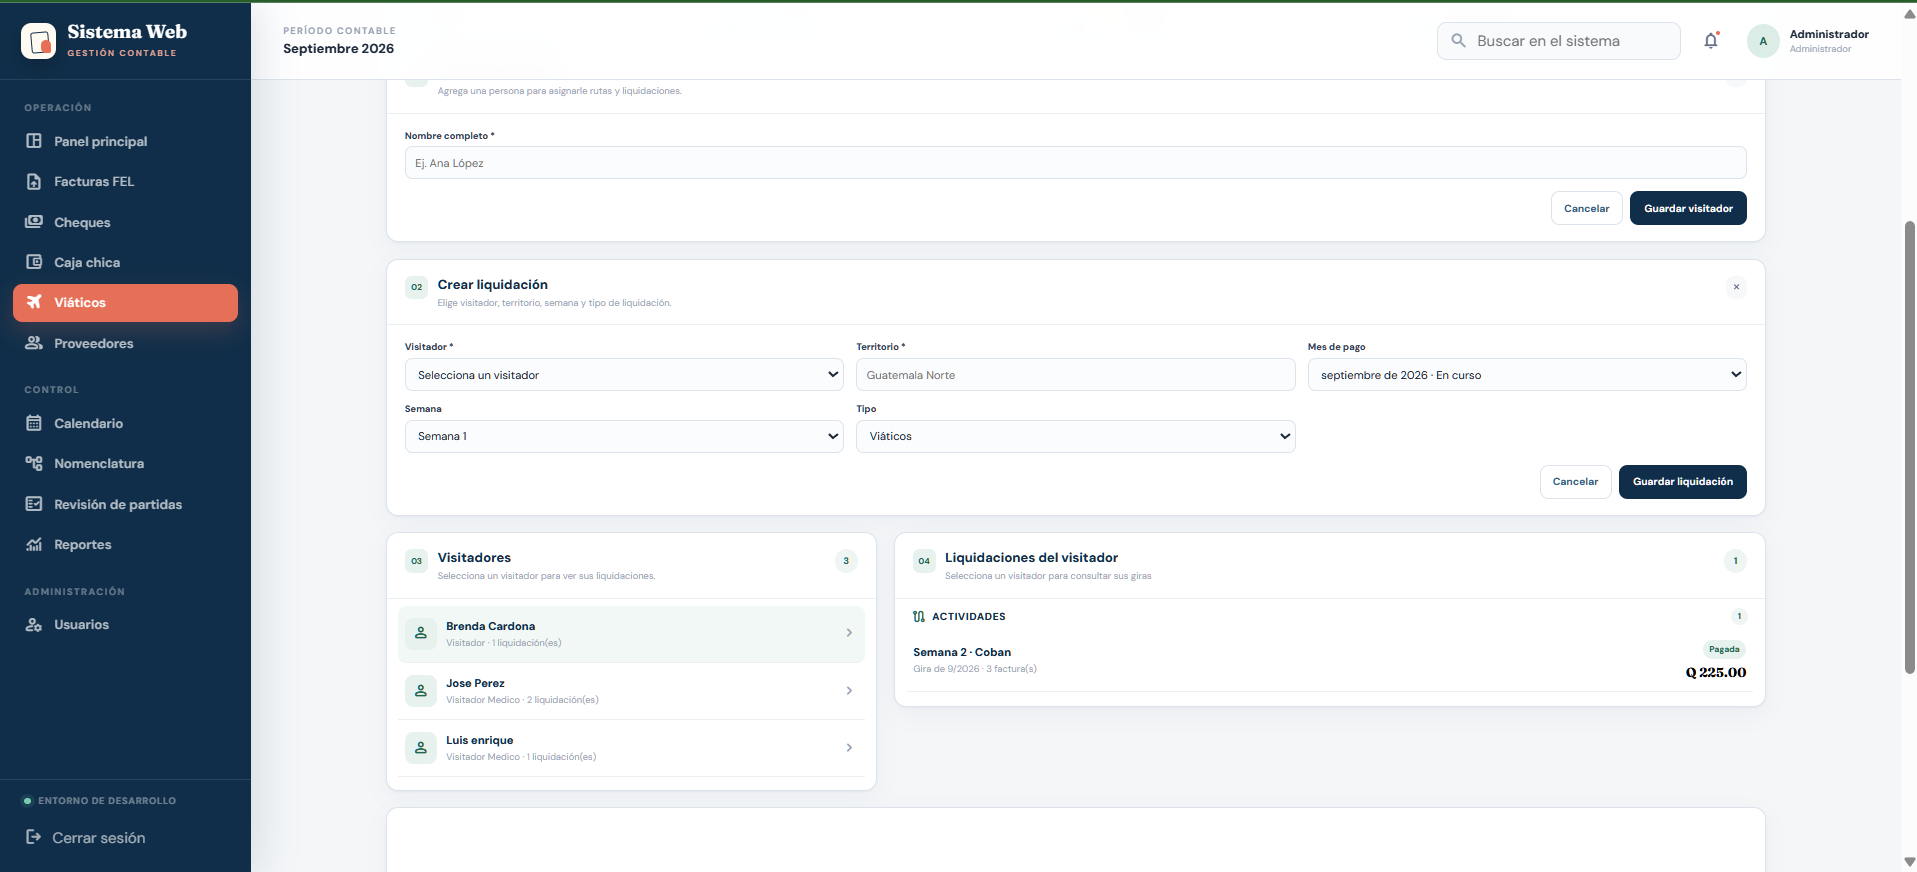
\includegraphics[width=0.96\linewidth]{capturas_reales/angular_actualizadas/pantalla_07_viaticos_nueva_liquidacion.png}
\end{figure}

% =========================================================================
% MÓDULO 5: PROVEEDORES
% =========================================================================
\subsubsection{Módulo: Proveedores}

{
\small
\setstretch{1.15}
\setlength{\parindent}{0pt}
\begin{xltabular}{\linewidth}{
    >{\raggedright\arraybackslash}p{1.3cm} 
    >{\raggedright\arraybackslash}p{2.2cm} 
    >{\raggedright\arraybackslash}>{\hsize=1.15\hsize}X 
    >{\raggedright\arraybackslash}>{\hsize=0.85\hsize}X 
    >{\centering\arraybackslash}p{0.6cm} 
    >{\raggedright\arraybackslash}p{2.0cm}
}

    % --- Encabezado de la primera página ---
    \caption{Resumen de formularios - Módulo: Proveedores} \label{tab:cap4_proveedores_resumen} \\
    \toprule
    \textbf{Código} & \textbf{Formulario} & \textbf{Propósito} & \textbf{Roles/Permisos} & \textbf{Op.} & \textbf{Ruta} \\
    \midrule
    \endfirsthead

    % --- Encabezado en páginas siguientes ---
    \toprule
    \textbf{Código} & \textbf{Formulario} & \textbf{Propósito} & \textbf{Roles/Permisos} & \textbf{Op.} & \textbf{Ruta} \\
    \midrule
    \endhead

    % --- Cierre en página intermedia ---
    \bottomrule
    \endfoot

    % --- Cierre final ---
    \bottomrule
    \endlastfoot

    % --- Filas de datos ---
    F-PROV-01 & Registro Proveedor & Alta por NIT, datos comerciales y condiciones de pago & Admin, Compras, Contador ({proveedores\_crear}) & C/U & {/proveedores} \\
    \addlinespace
    F-PROV-02 & Cartera y Facturas & Consultar saldos, crédito, retenciones e historial & Admin, Contador ({proveedores\_ver}) & R & {/proveedores} \\
    \addlinespace
    F-PROV-03 & Generación Partida & Crear partida dentro del mes o transitoria & Admin, Contador ({proveedores\_partida}) & C & {/proveedores} \\

\end{xltabular}
}

\paragraph{Formulario F-PROV-01: Registro y Configuración de Proveedores}
\noindent\textbf{Objetivo:} Crear y mantener el registro maestro de proveedores con su NIT, nombre comercial, retenciones autorizadas y cuenta contable por defecto. \\[0.3em]
\textbf{Ubicación / Ruta:} Módulo Proveedores $\rightarrow$ Nuevo proveedor ({/proveedores}). \\[0.3em]
\textbf{Roles/Permisos:} Admin, Compras, Contador ({proveedores\_crear}). \\[0.3em]
\textbf{Campos clave y validaciones críticas:} {nit\_proveedor} (Requerido, único, formato tributario guatemalteco); {nombre\_comercial} y {razon\_social} (Requeridos); {dias\_credito} (Integer $\ge 0$, ej.: 30 días); {aplica\_retencion\_isr} / {iva} (Boolean); {cuenta\_nomenclatura\_id} (Requerido, enlace a Nomenclatura Contable). \\[0.3em]
\textbf{Flujo:} Hacer clic en ``Nuevo proveedor'' $\rightarrow$ Ingresar NIT para autocompletado/verificación $\rightarrow$ Asignar cuenta contable y condiciones de crédito $\rightarrow$ Guardar registro. \\[0.3em]
\textbf{Mensaje principal del sistema:} ``Proveedor registrado exitosamente.''

\begin{figure}[H]
    \centering
    \caption{Módulo de Proveedores con cartera de crédito y gestión de partidas.}
    \label{fig:cap4_proveedores_pantalla}
    \vspace{0.2cm}
    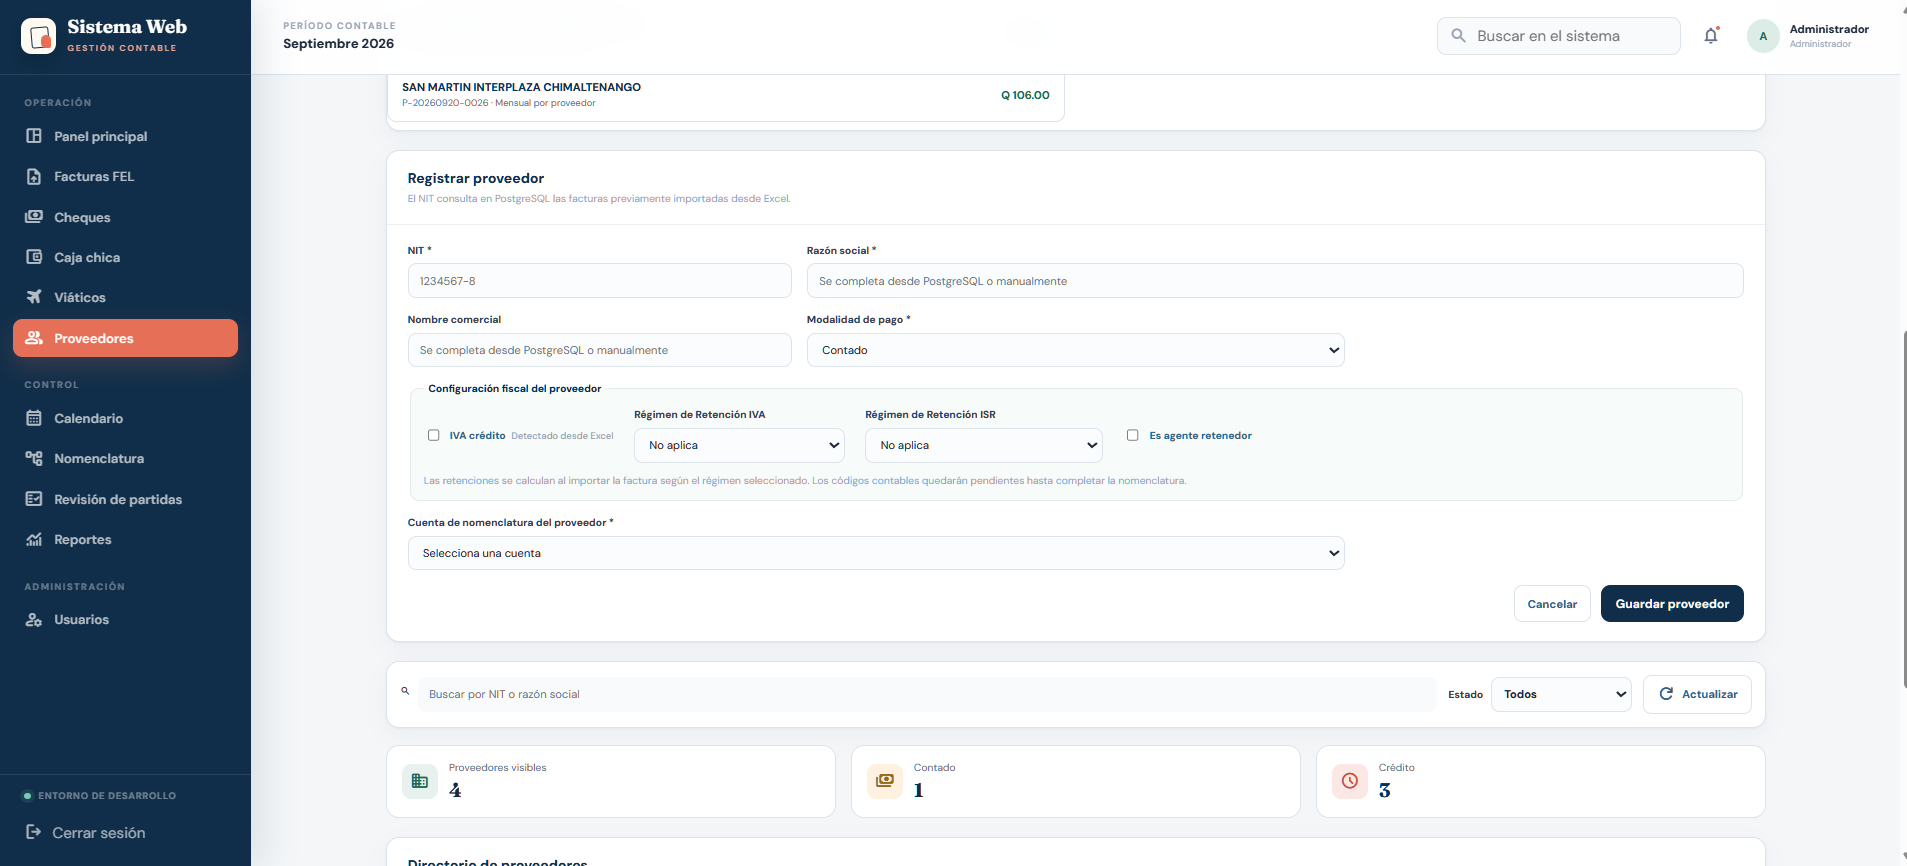
\includegraphics[width=0.96\linewidth]{capturas_reales/angular_actualizadas/pantalla_08_proveedores_nuevo.png}
\end{figure}

% =========================================================================
% MÓDULO 6: CALENDARIO OPERATIVO
% =========================================================================
\subsubsection{Módulo: Calendario Operativo}

{
\small
\setstretch{1.15}
\setlength{\parindent}{0pt}
\begin{xltabular}{\linewidth}{
    >{\raggedright\arraybackslash}p{1.3cm} 
    >{\raggedright\arraybackslash}p{2.2cm} 
    >{\raggedright\arraybackslash}>{\hsize=1.15\hsize}X 
    >{\raggedright\arraybackslash}>{\hsize=0.85\hsize}X 
    >{\centering\arraybackslash}p{0.6cm} 
    >{\raggedright\arraybackslash}p{2.0cm}
}

    % --- Encabezado de la primera página ---
    \caption{Resumen de formularios - Módulo: Calendario Operativo} \label{tab:cap4_calendario_resumen} \\
    \toprule
    \textbf{Código} & \textbf{Formulario} & \textbf{Propósito} & \textbf{Roles/Permisos} & \textbf{Op.} & \textbf{Ruta} \\
    \midrule
    \endfirsthead

    % --- Encabezado en páginas siguientes ---
    \toprule
    \textbf{Código} & \textbf{Formulario} & \textbf{Propósito} & \textbf{Roles/Permisos} & \textbf{Op.} & \textbf{Ruta} \\
    \midrule
    \endhead

    % --- Cierre en página intermedia ---
    \bottomrule
    \endfoot

    % --- Cierre final ---
    \bottomrule
    \endlastfoot

    % --- Filas de datos ---
    F-CAL-01 & Vista Calendario & Consultar eventos, pagos, depósitos y giras & Todos ({calendario\_ver}) & R & {/calendario} \\
    \addlinespace
    F-CAL-02 & Evento / Actividad & Programar nueva actividad contable u operativa & Admin, Encargado ({calendario\_crear}) & C/U & {/calendario} \\

\end{xltabular}
}

\paragraph{Formulario F-CAL-02: Programación de Actividades y Eventos}
\noindent\textbf{Objetivo:} Programar eventos financieros como fechas de depósito de cheques posfechados, vencimiento de facturas de proveedores o inicio de giras. \\[0.3em]
\textbf{Ubicación / Ruta:} Módulo Calendario $\rightarrow$ Nueva Actividad ({/calendario}). \\[0.3em]
\textbf{Roles/Permisos:} Admin, Encargado ({calendario\_crear}). \\[0.3em]
\textbf{Campos clave y validaciones críticas:} {titulo\_evento} (Requerido, ej.: ``Pago Proveedor Distribuidora X''); {fecha\_inicio} y {fecha\_fin} (Requeridas, {fecha\_fin} $\ge$ {fecha\_inicio}); {tipo\_actividad} (Requerido: Pago, Cheque, Gira, Auditoría); {prioridad} (Alta, Media, Baja). \\[0.3em]
\textbf{Flujo:} Seleccionar fecha en el calendario o presionar ``Actividad'' $\rightarrow$ Llenar detalles del evento $\rightarrow$ Guardar $\rightarrow$ Actualización dinámica en el calendario. \\[0.3em]
\textbf{Mensaje principal del sistema:} ``Evento agregado al calendario operativo.''

\begin{figure}[H]
    \centering
    \caption{Módulo de Calendario Operativo con eventos y vencimientos anotados.}
    \label{fig:cap4_calendario_pantalla}
    \vspace{0.2cm}
    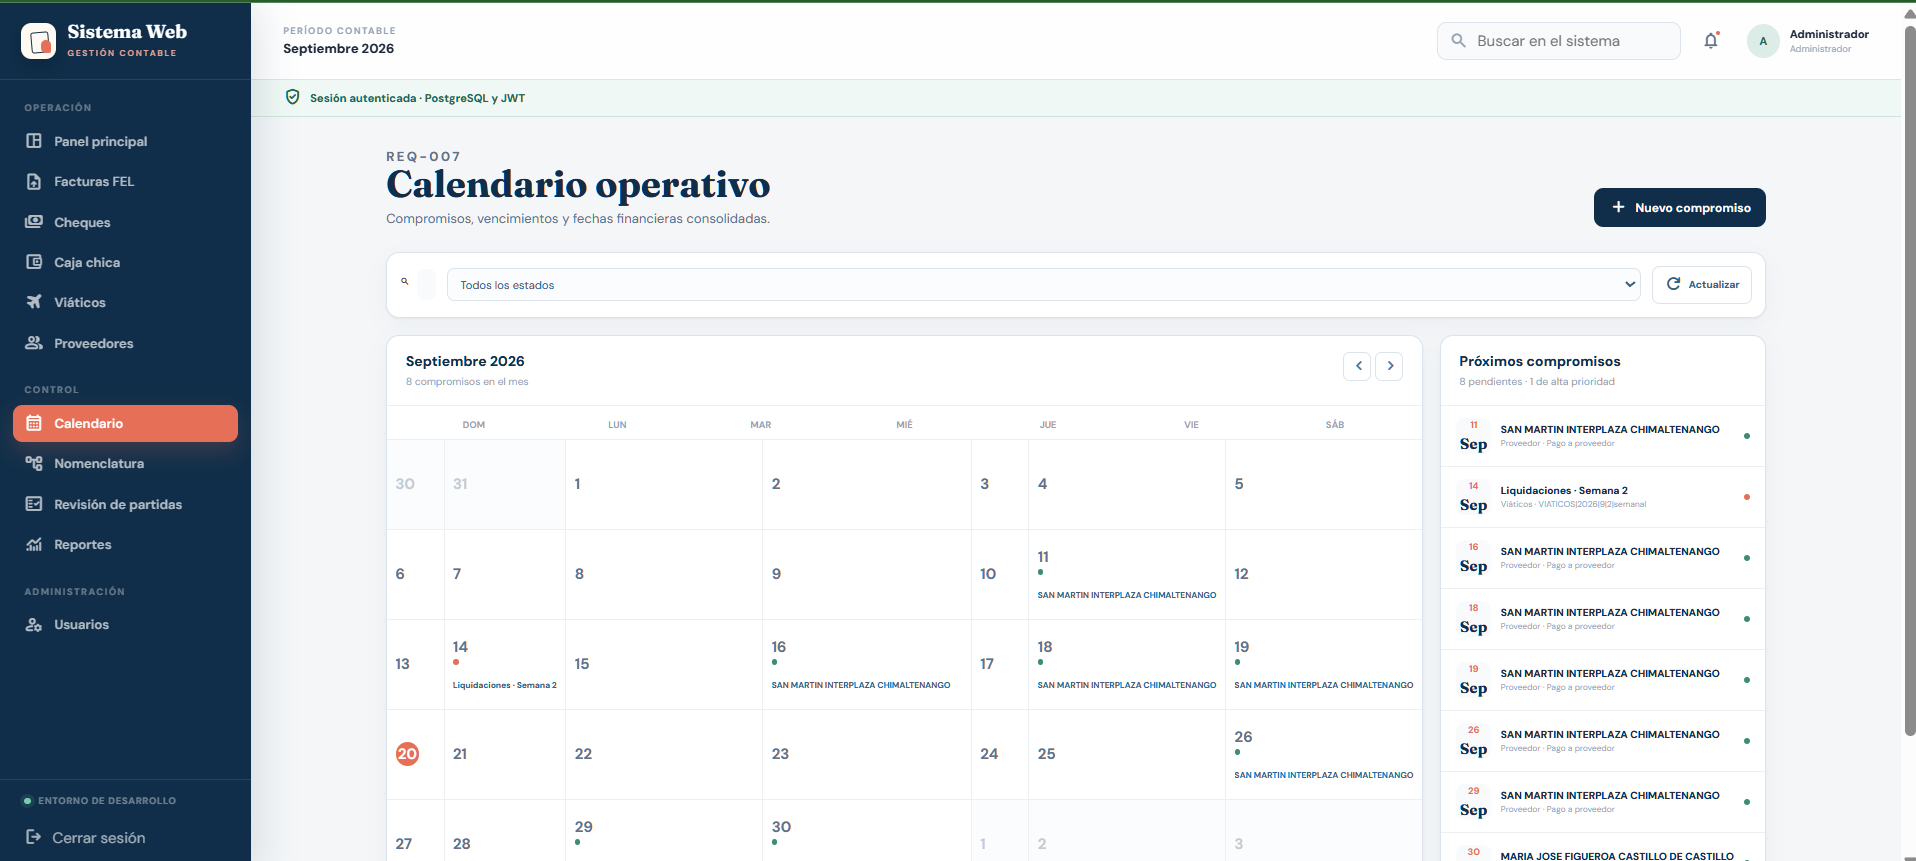
\includegraphics[width=0.96\linewidth]{capturas_reales/angular_actualizadas/pantalla_09_calendario.png}
\end{figure}

% =========================================================================
% MÓDULO 7: NOMENCLATURA CONTABLE
% =========================================================================
\subsubsection{Módulo: Nomenclatura Contable}

{
\small
\setstretch{1.15}
\setlength{\parindent}{0pt}
\begin{xltabular}{\linewidth}{
    >{\raggedright\arraybackslash}p{1.3cm} 
    >{\raggedright\arraybackslash}p{2.2cm} 
    >{\raggedright\arraybackslash}>{\hsize=1.15\hsize}X 
    >{\raggedright\arraybackslash}>{\hsize=0.85\hsize}X 
    >{\centering\arraybackslash}p{0.6cm} 
    >{\raggedright\arraybackslash}p{2.0cm}
}

    % --- Encabezado de la primera página ---
    \caption{Resumen de formularios - Módulo: Nomenclatura Contable} \label{tab:cap4_nomenclatura_resumen} \\
    \toprule
    \textbf{Código} & \textbf{Formulario} & \textbf{Propósito} & \textbf{Roles/Permisos} & \textbf{Op.} & \textbf{Ruta} \\
    \midrule
    \endfirsthead

    % --- Encabezado en páginas siguientes ---
    \toprule
    \textbf{Código} & \textbf{Formulario} & \textbf{Propósito} & \textbf{Roles/Permisos} & \textbf{Op.} & \textbf{Ruta} \\
    \midrule
    \endhead

    % --- Cierre en página intermedia ---
    \bottomrule
    \endfoot

    % --- Cierre final ---
    \bottomrule
    \endlastfoot

    % --- Filas de datos ---
    F-NOM-01 & Catálogo Cuentas & Listar, buscar y filtrar catálogo de cuentas & Admin, Contador ({nomenclatura\_ver}) & R & {/nomenclatura} \\
    \addlinespace
    F-NOM-02 & Formulario Cuenta & Crear o editar código, nombre y naturaleza de cuenta & Admin, Contador ({nomenclatura\_crear}) & C/U & {/nomenclatura} \\

\end{xltabular}
}

\paragraph{Formulario F-NOM-02: Formulario de Cuenta Contable}
\noindent\textbf{Objetivo:} Crear y actualizar la estructura del plan de cuentas (Nomenclatura) indicando el código jerárquico y la naturaleza contable (Debe / Haber). \\[0.3em]
\textbf{Ubicación / Ruta:} Nomenclatura $\rightarrow$ Nueva Cuenta / Editar ({/nomenclatura}). \\[0.3em]
\textbf{Roles/Permisos:} Admin, Contador ({nomenclatura\_crear}). \\[0.3em]
\textbf{Campos clave y validaciones críticas:} {codigo\_cuenta} (Requerido, único, formato estructurado, ej.: {5.1.01.001}); {nombre\_cuenta} (Requerido, ej.: ``Gastos de Operación'').

\subsubsection{Módulo: Autenticación y Gestión de Usuarios}
La Tabla~\ref{tab:cap4_auth_resumen} resume el formulario de acceso y la administración de credenciales y roles.

{
\small
\setstretch{1.15}
\setlength{\parindent}{0pt}
\begin{xltabular}{\linewidth}{
    >{\raggedright\arraybackslash}p{1.3cm} 
    >{\raggedright\arraybackslash}p{2.2cm} 
    >{\raggedright\arraybackslash}>{\hsize=1.15\hsize}X 
    >{\raggedright\arraybackslash}>{\hsize=0.85\hsize}X 
    >{\centering\arraybackslash}p{0.6cm} 
    >{\raggedright\arraybackslash}p{2.0cm}
}
\caption{Resumen de formularios - Módulo: Autenticación y gestión de usuarios}\label{tab:cap4_auth_resumen}\\
\toprule
\textbf{Código} & \textbf{Formulario} & \textbf{Propósito} & \textbf{Roles/Permisos} & \textbf{Op.} & \textbf{Ruta}\\
\midrule
\endfirsthead
\toprule
\textbf{Código} & \textbf{Formulario} & \textbf{Propósito} & \textbf{Roles/Permisos} & \textbf{Op.} & \textbf{Ruta}\\
\midrule
\endhead
\bottomrule
\endfoot
\bottomrule
\endlastfoot
F-AUTH-01 & Inicio de sesión & Validar credenciales y habilitar la sesión autorizada & Usuario registrado ({iniciar\_sesion}) & C/R & {/login}\\
\addlinespace
F-AUTH-02 & Usuarios y roles & Registrar usuarios y asignar permisos de acceso & Admin ({gestionar\_usuarios}) & CRUD & {/usuarios}\\
\end{xltabular}
}

\paragraph{Formulario F-AUTH-01: Inicio de sesión}
\noindent\textbf{Objetivo:} Validar el usuario y la contraseña antes de permitir el acceso al Panel principal. \textbf{Campos y validaciones:} usuario requerido, contraseña requerida y mensaje controlado para credenciales inválidas. \textbf{Flujo:} ingresar credenciales $\rightarrow$ presionar ``Ingresar al sistema'' $\rightarrow$ validar sesión $\rightarrow$ mostrar el Panel principal.

\begin{figure}[H]
    \centering
    \caption{Pantalla de inicio de sesión del sistema.}
    \label{fig:cap4_auth_pantalla}
    
\includegraphics[width=0.96\linewidth]{capturas_reales/angular_actualizadas/pantalla_01_login.png}
\end{figure}

\subsubsection{Módulo: Reportes Operativos y Financieros}
La Tabla~\ref{tab:cap4_reportes_resumen} documenta las funciones de consulta y generación de reportes autorizados.

{
\small
\setstretch{1.15}
\setlength{\parindent}{0pt}
\begin{xltabular}{\linewidth}{
    >{\raggedright\arraybackslash}p{1.3cm} 
    >{\raggedright\arraybackslash}p{2.2cm} 
    >{\raggedright\arraybackslash}>{\hsize=1.15\hsize}X 
    >{\raggedright\arraybackslash}>{\hsize=0.85\hsize}X 
    >{\centering\arraybackslash}p{0.6cm} 
    >{\raggedright\arraybackslash}p{2.0cm}
}
\caption{Resumen de formularios - Módulo: Reportes operativos y financieros}\label{tab:cap4_reportes_resumen}\\
\toprule
\textbf{Código} & \textbf{Formulario} & \textbf{Propósito} & \textbf{Roles/Permisos} & \textbf{Op.} & \textbf{Ruta}\\
\midrule
\endfirsthead
\toprule
\textbf{Código} & \textbf{Formulario} & \textbf{Propósito} & \textbf{Roles/Permisos} & \textbf{Op.} & \textbf{Ruta}\\
\midrule
\endhead
\bottomrule
\endfoot
\bottomrule
\endlastfoot
F-REP-01 & Consulta de reportes & Filtrar información por período, módulo y estado & Admin, Contador ({consultar\_reportes}) & R & {/reportes}\\
\addlinespace
F-REP-02 & Resumen de Caja chica & Revisar e imprimir los movimientos del fondo & Admin, Contador ({consultar\_caja}) & R & {/reportes/caja-chica}\\
\end{xltabular}
}

\paragraph{Formulario F-REP-01: Consulta de reportes}
\noindent\textbf{Objetivo:} Presentar información consolidada para revisión operativa y financiera. \textbf{Campos y validaciones:} período requerido, módulo opcional y estado válido. \textbf{Flujo:} seleccionar filtros $\rightarrow$ consultar $\rightarrow$ revisar resultados $\rightarrow$ imprimir o guardar el reporte autorizado.

\begin{figure}[H]
    \centering
    \caption{Pantalla de reportes operativos y financieros.}
    \label{fig:cap4_reportes_pantalla}
    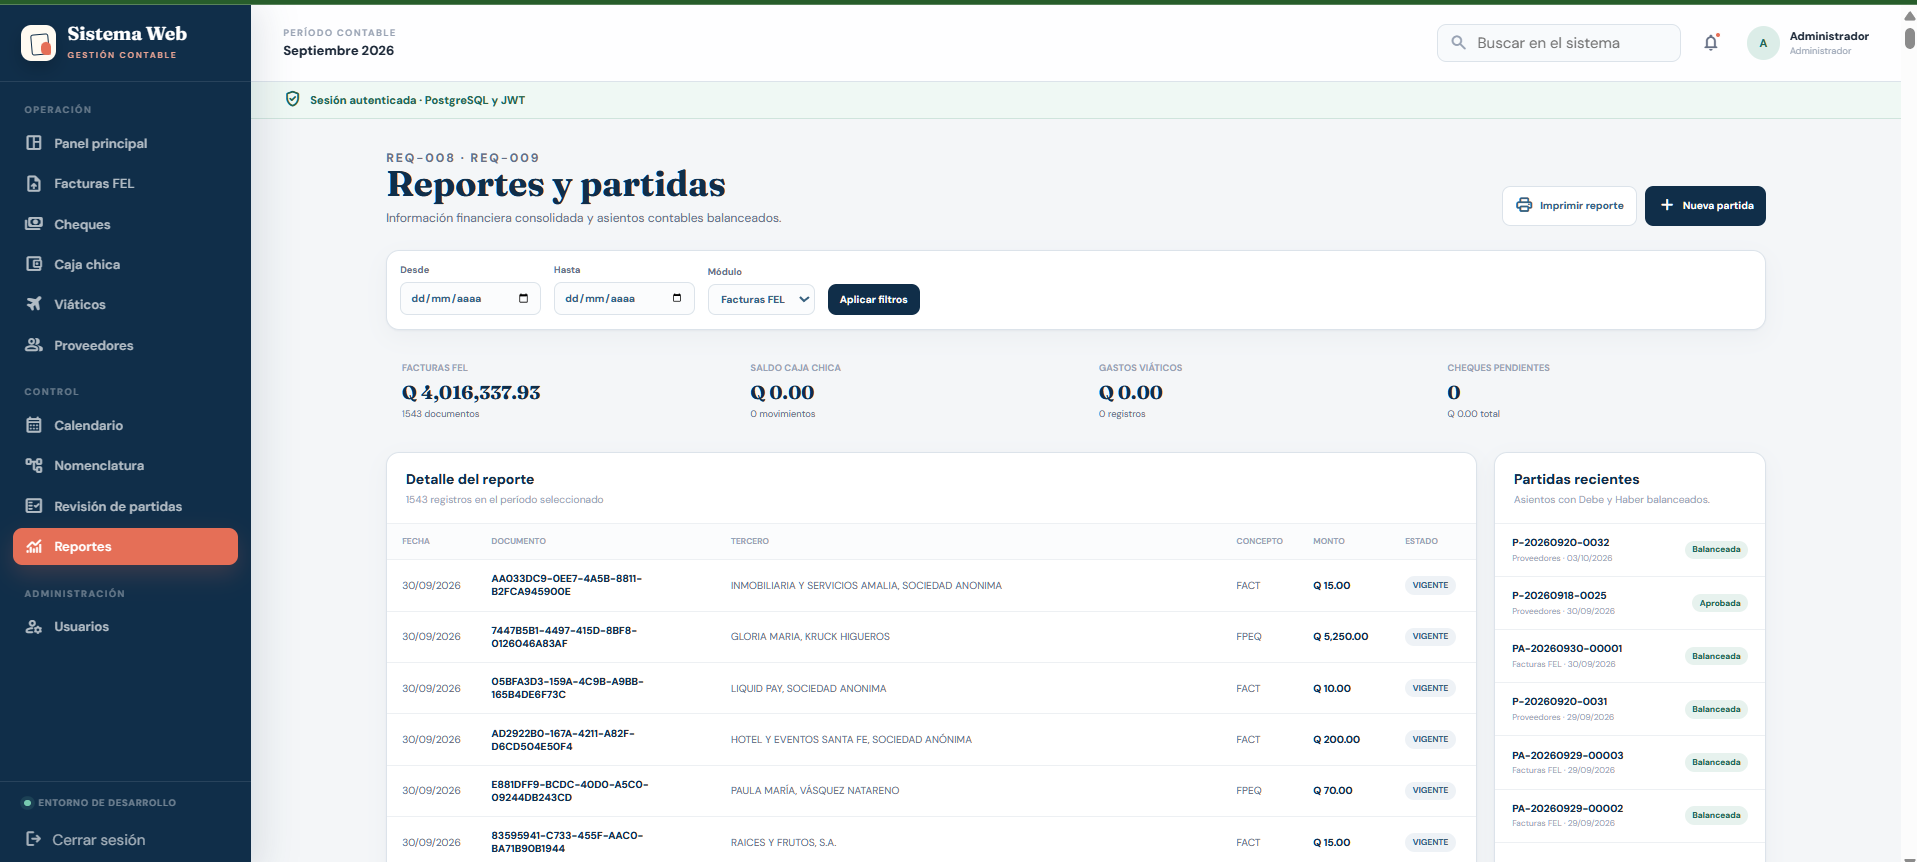
\includegraphics[width=0.96\linewidth]{capturas_reales/angular_actualizadas/pantalla_11_reportes.png}
\end{figure}

\subsection{Fragmentos de Código}
\label{sec:cap4_fragmentos_codigo}

De conformidad con los lineamientos metodológicos, en este apartado se documenta el desarrollo técnico del sistema mediante ocho fragmentos representativos y demostrativos de código fuente, preparados para ilustrar la lógica correspondiente a cada módulo. Cada extracto incluye su especificación de módulo, lenguaje utilizado, bloque de código en fuente monoespaciada, descripción funcional y la evidencia correspondiente a la interfaz de usuario real.

% =========================================================================
% FRAGMENTO 1: FACTURAS FEL (PYTHON/FASTAPI)
% =========================================================================
\subsubsection{Fragmento 1: Procesamiento y Validación de DTE FEL}
\noindent\textbf{Módulo:} Facturas FEL/SAT \\
\textbf{Lenguaje:} Python (FastAPI)

A continuación, se presenta el fragmento de código encargado de procesar la estructura XML de las facturas electrónicas y verificar la no duplicidad del UUID tributario:

\begin{minted}[breaklines, fontsize=\normalsize]{python}
@router.post("/importar-xml")
async def importar_xml_fel(file: UploadFile = File(...), db: Session = Depends(get_db)):
    if not file.filename.endswith('.xml'):
        raise HTTPException(status_code=400, detail="Formato de archivo invalido")
    
    content = await file.read()
    tree = ET.fromstring(content)
    uuid_dte = tree.find(".//{http://www.sat.gob.gt/dte/fel/0.1.0}NumeroAutorizacion").text
    
    existe = db.query(FacturaFEL).filter(FacturaFEL.uuid == uuid_dte).first()
    if existe:
        raise HTTPException(status_code=400, detail="El DTE ya se encuentra registrado")
    
    nueva_factura = FacturaFEL(uuid=uuid_dte, estado="PENDIENTE")
    db.add(nueva_factura)
    db.commit()
    return {"status": "exito", "uuid": uuid_dte}
\end{minted}

\noindent\textbf{Descripción:} Este código pertenece al backend del módulo de Facturas FEL/SAT. Su función principal es recibir la carga de archivos XML, analizar el árbol DOM para extraer el UUID oficial emitido por la SAT y validar en la base de datos que el documento no haya sido ingresado previamente.

\begin{figure}[H]
    \centering
    \caption{Formulario de carga masiva e importación de comprobantes FEL.}
    \label{fig:cap4_code_fel_xml}
    \vspace{0.2cm}
    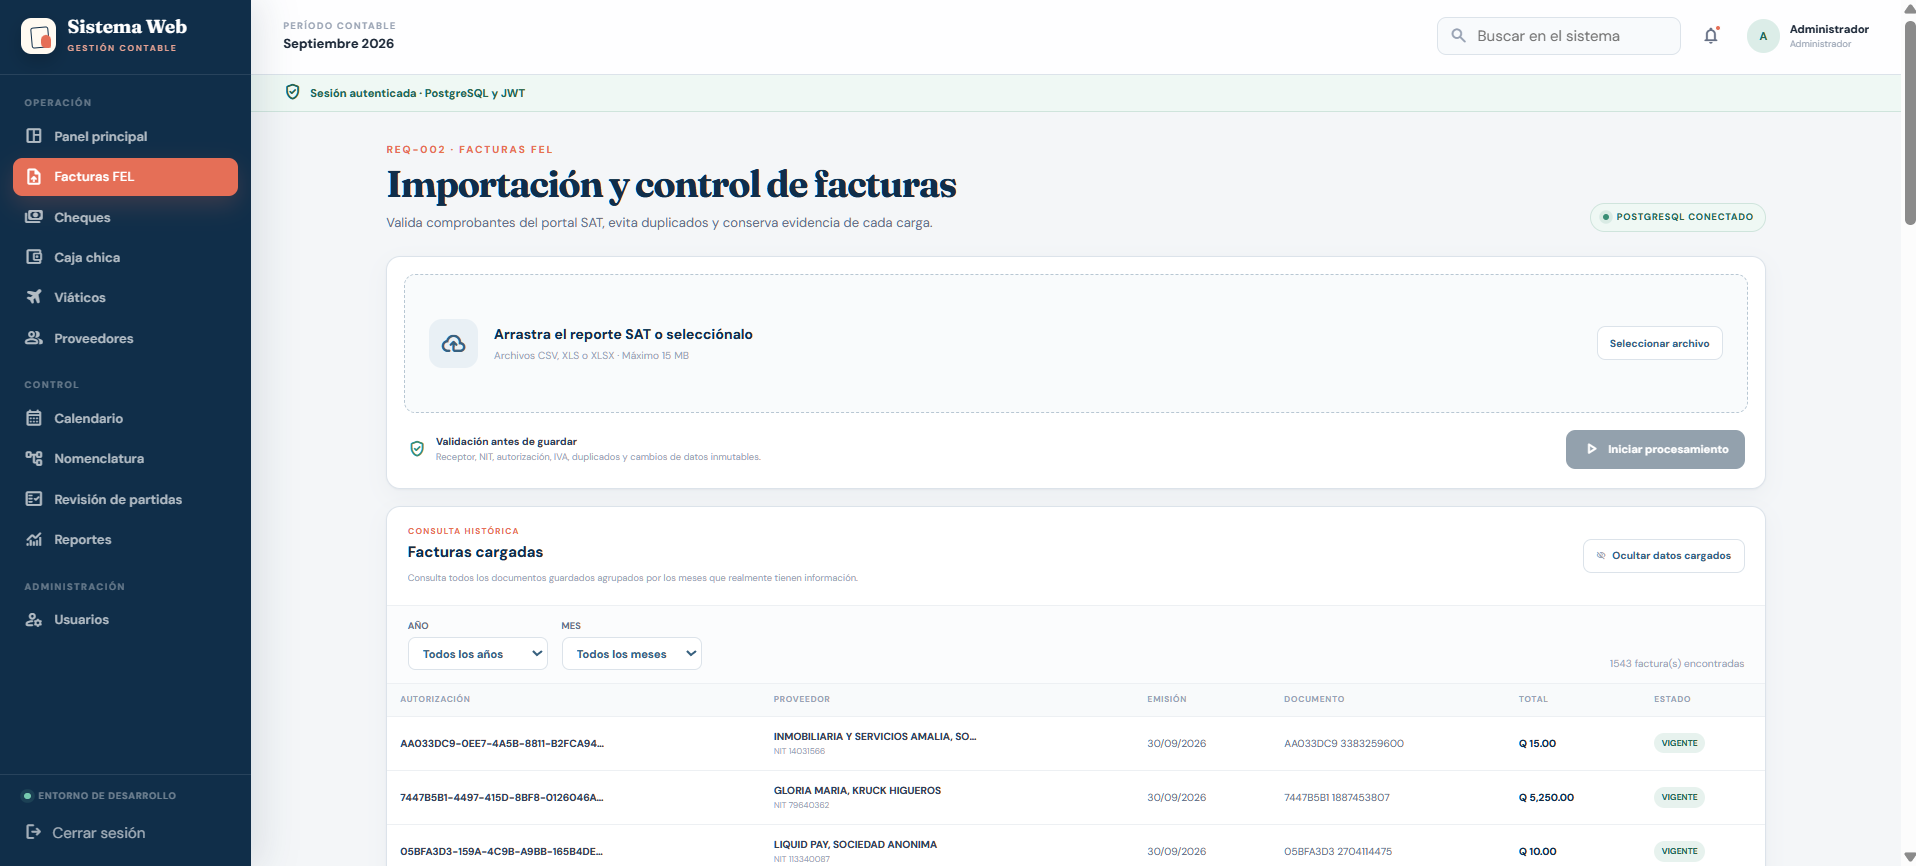
\includegraphics[width=0.96\linewidth]{capturas_reales/angular_actualizadas/pantalla_03_facturas_fel.png}
    \vspace{0.1cm}
    \begin{minipage}{0.96\linewidth}
        \small\textit{Nota.} La captura de pantalla corresponde al formulario web real que consume el endpoint de validación de archivos XML.
    \end{minipage}
\end{figure}

% =========================================================================
% FRAGMENTO 2: CHEQUES POSFECHADOS (PYTHON/FASTAPI)
% =========================================================================
\subsubsection{Fragmento 2: Registro y Validación de Cheques Posfechados}
\noindent\textbf{Módulo:} Cheques Posfechados \\
\textbf{Lenguaje:} Python (FastAPI)

A continuación, se presenta la lógica de validación de fechas y montos en el registro de cheques posfechados:

\begin{minted}[breaklines, fontsize=\small]{python}
@router.post("/cheques")
def crear_cheque(cheque: ChequeCreate, db: Session = Depends(get_db)):
    if cheque.fecha_deposito < cheque.fecha_recepcion:
        raise HTTPException(status_code=400, detail="La fecha de deposito debe ser mayor o igual a la de recepcion")
    
    if cheque.monto <= 0:
        raise HTTPException(status_code=400, detail="El monto del cheque debe ser mayor a cero")
        
    nuevo_cheque = Cheque(**cheque.dict(), estado="PENDIENTE")
    db.add(nuevo_cheque)
    db.commit()
    db.refresh(nuevo_cheque)
    return nuevo_cheque
\end{minted}

\noindent\textbf{Descripción:} El fragmento corresponde a la capa de servicios del módulo de Cheques Posfechados. Garantiza la coherencia cronológica de las fechas de depósito respecto a las de recepción y asegura que únicamente se registren montos financieros válidos antes de persistir la información.

\begin{figure}[H]
    \centering
    \caption{Formulario de gestión e ingreso de cheques posfechados.}
    \label{fig:cap4_code_cheques}
    \vspace{0.2cm}
    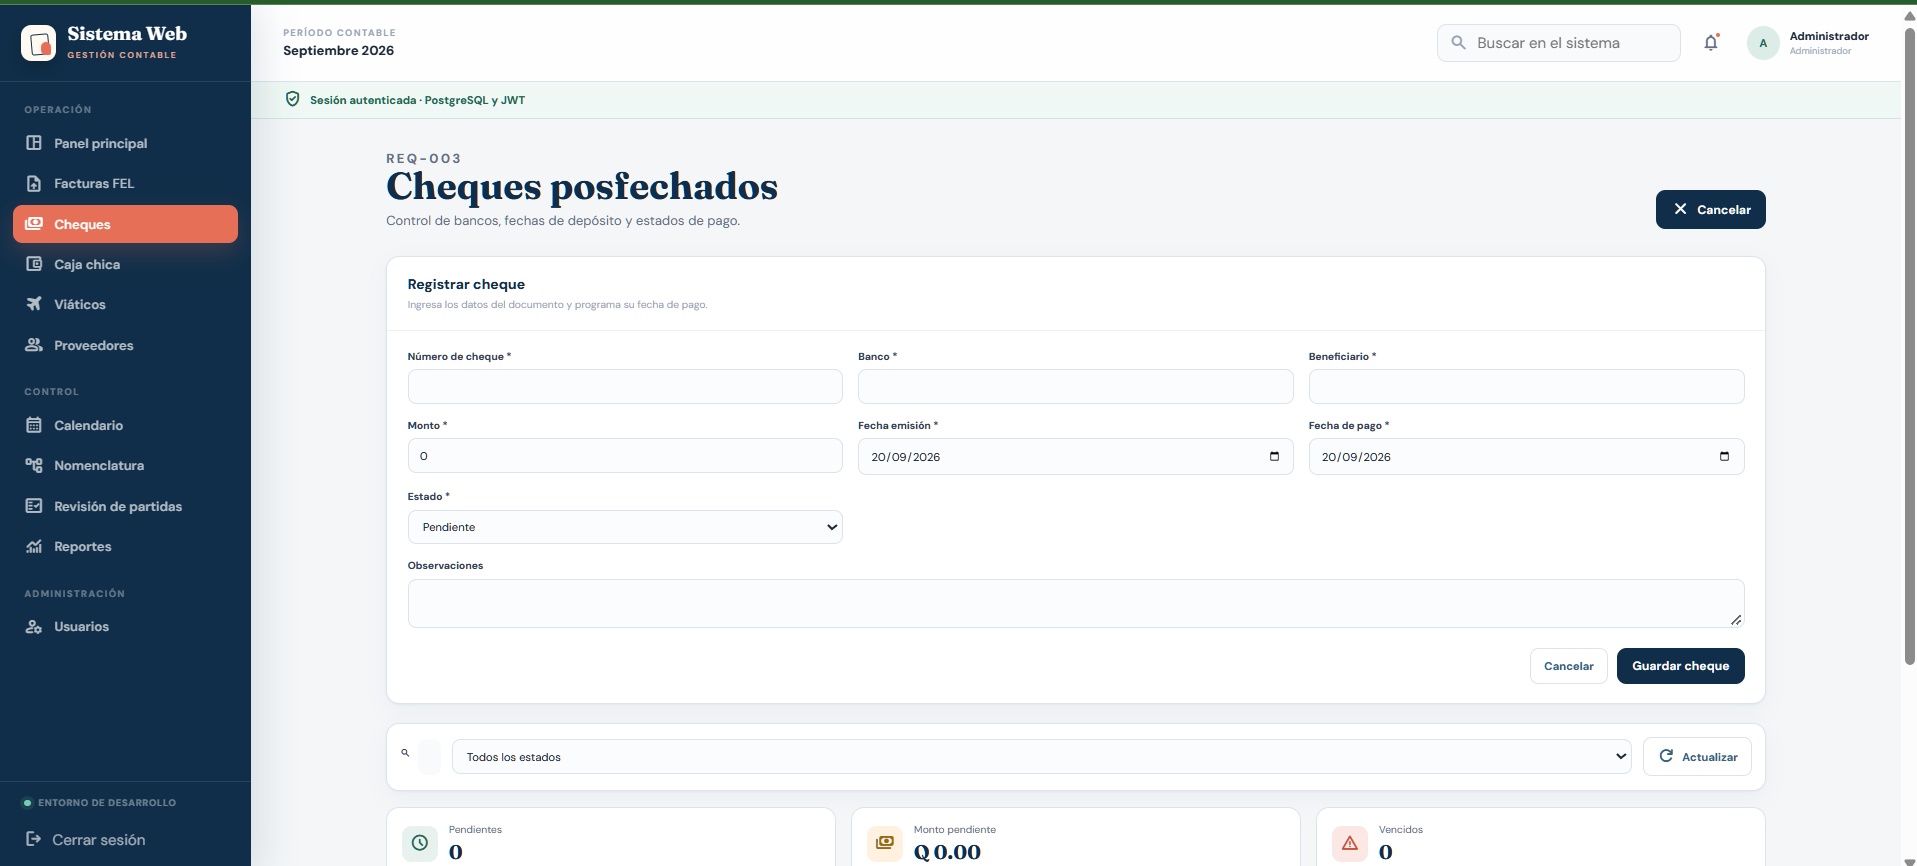
\includegraphics[width=0.96\linewidth]{capturas_reales/angular_actualizadas/formulario_cheque.png}
    \vspace{0.1cm}
    \begin{minipage}{0.96\linewidth}
        \small\textit{Nota.} La captura de pantalla ilustra la interfaz de registro de cheques respaldada por el método de verificación en backend.
    \end{minipage}
\end{figure}

% =========================================================================
% FRAGMENTO 3: CAJA CHICA (PYTHON/FASTAPI)
% =========================================================================
\subsubsection{Fragmento 3: Control de Disponible y Registro de Egresos}
\noindent\textbf{Módulo:} Caja Chica \\
\textbf{Lenguaje:} Python (FastAPI)

A continuación, se expone la función encargada de verificar la disponibilidad de saldo en el fondo fijo previo al registro de un recibo de egreso:

\begin{minted}[breaklines, fontsize=\small]{python}
@router.post("/caja-chica/recibo")
def registrar_recibo(recibo: ReciboCreate, db: Session = Depends(get_db)):
    fondo = db.query(FondoCajaChica).filter(FondoCajaChica.activo == True).first()
    if not fondo:
        raise HTTPException(status_code=404, detail="No existe un fondo de caja chica activo")
        
    if recibo.monto_total > fondo.saldo_disponible:
        raise HTTPException(status_code=400, detail="El monto excede el saldo disponible del fondo")
        
    fondo.saldo_disponible -= recibo.monto_total
    nuevo_movimiento = MovimientoCaja(**recibo.dict(), fondo_id=fondo.id)
    db.add(nuevo_movimiento)
    db.commit()
    return nuevo_movimiento
\end{minted}

\noindent\textbf{Descripción:} Este código corresponde a la lógica de negocio de Caja Chica. Evalúa que la caja posea saldo suficiente para cubrir el gasto solicitado y efectúa el débito automático sobre el fondo asignado al momento de guardar el recibo.

\begin{figure}[H]
    \centering
    \caption{Formulario para captura de recibos y egresos de Caja Chica.}
    \label{fig:cap4_code_caja}
    \vspace{0.2cm}
    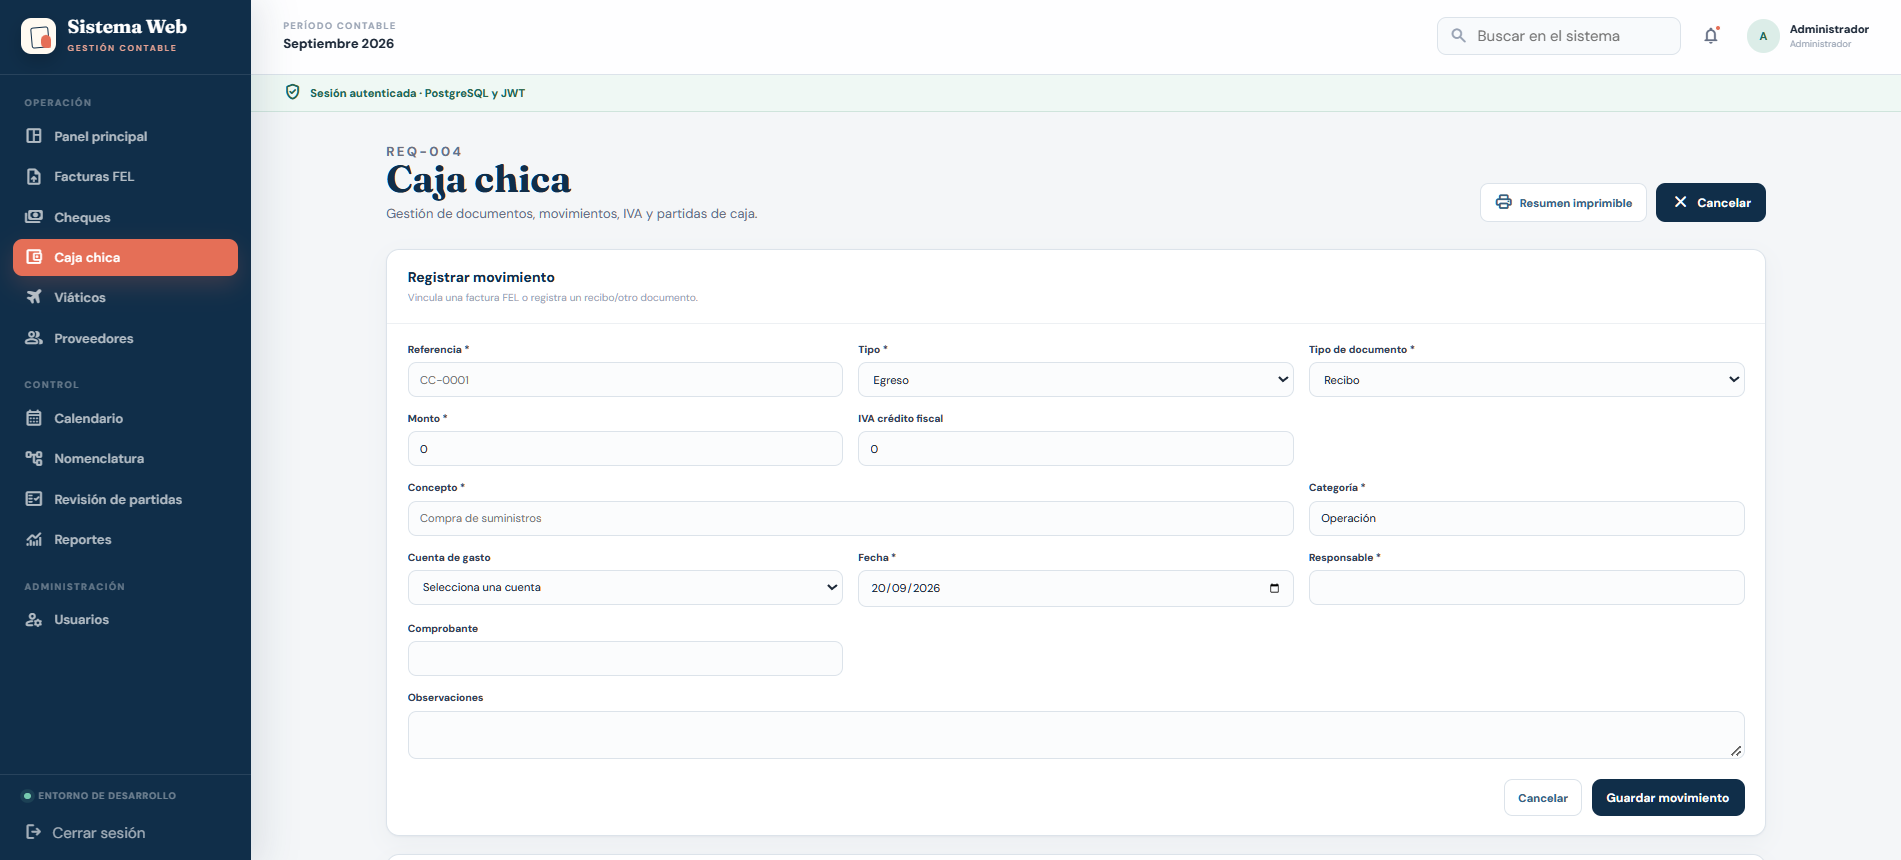
\includegraphics[width=0.96\linewidth]{capturas_reales/angular_actualizadas/formulario_caja_chica.png}
    \vspace{0.1cm}
    \begin{minipage}{0.96\linewidth}
        \small\textit{Nota.} La captura muestra la pantalla interactiva de la caja chica donde el usuario liquida recibos bajo la regla de saldo disponible.
    \end{minipage}
\end{figure}

% =========================================================================
% FRAGMENTO 4: VIÁTICOS (TYPESCRIPT/ANGULAR)
% =========================================================================
\subsubsection{Fragmento 4: Regla de Asignación por Categoría de Viático}
\noindent\textbf{Módulo:} Viáticos \\
\textbf{Lenguaje:} TypeScript (Angular)

A continuación, se muestra el método de validación en frontend para restringir categorías de gastos según el calendario operativo de la gira:

\begin{minted}[breaklines, fontsize=\small]{python}
validarCategoriaGasto(semanaGira: number, categoriaSeleccionada: string): boolean {
  if (categoriaSeleccionada === 'MOVILIDAD' && semanaGira !== 1) {
    this.toastr.warning('La categoria Movilidad solo esta permitida durante la primera semana');
    this.formularioAsignacion.get('categoria_gasto')?.setValue('');
    return false;
  }
  return true;
}
\end{minted}

\noindent\textbf{Descripción:} El fragmento forma parte de la lógica del componente frontend en el módulo de Viáticos. Ejecuta una validación reactiva que prohíbe la selección de rubros de movilidad fuera de la primera semana operativa del mes, alertando al usuario mediante notificaciones.

\begin{figure}[H]
    \centering
    \caption{Formulario de asignación de facturas a giras y categorías de viáticos.}
    \label{fig:cap4_code_viaticos}
    \vspace{0.2cm}
    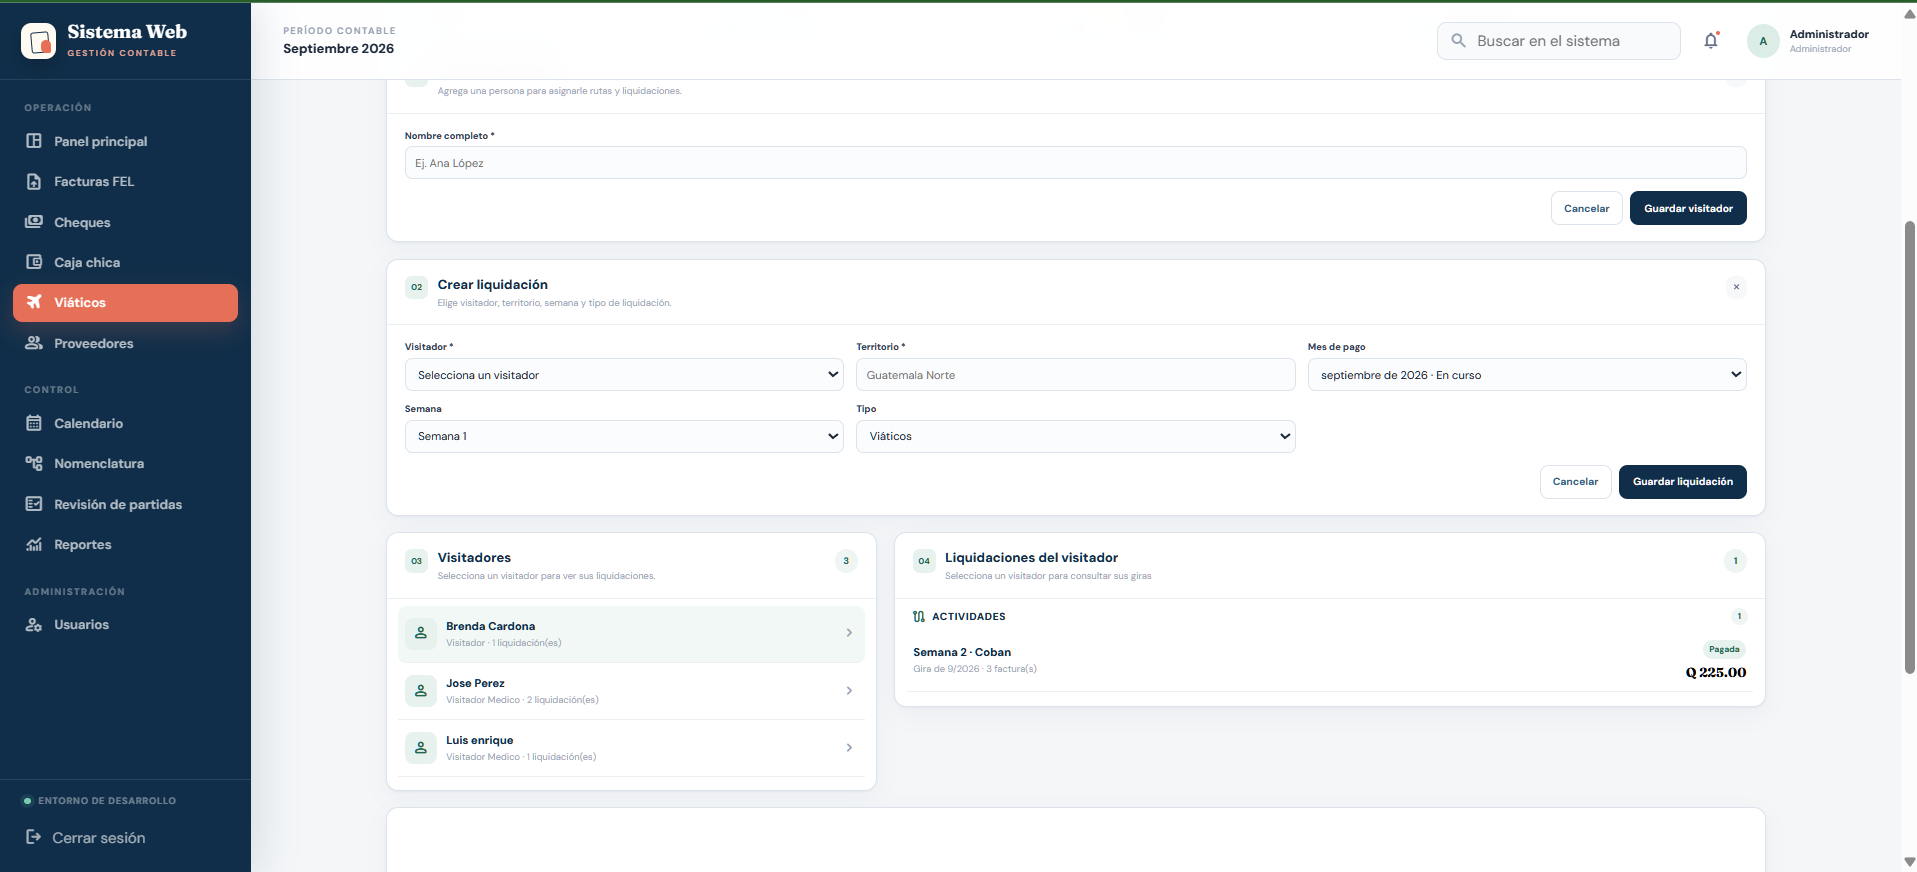
\includegraphics[width=0.96\linewidth]{capturas_reales/angular_actualizadas/pantalla_07_viaticos_nueva_liquidacion.png}
    \vspace{0.1cm}
    \begin{minipage}{0.96\linewidth}
        \small\textit{Nota.} Captura de la interfaz de asignación de viáticos operada bajo controles reactivos de TypeScript.
    \end{minipage}
\end{figure}

% =========================================================================
% FRAGMENTO 5: PROVEEDORES (PYTHON/FASTAPI)
% =========================================================================
\subsubsection{Fragmento 5: Alta de Proveedores y Asociación Contable}
\noindent\textbf{Módulo:} Proveedores \\
\textbf{Lenguaje:} Python (FastAPI)

A continuación, se presenta la función de creación de proveedores con verificación de formato tributario y asignación de cuenta por defecto:

\begin{minted}[breaklines, fontsize=\small]{python}
@router.post("/proveedores")
def registrar_proveedor(prov: ProveedorCreate, db: Session = Depends(get_db)):
    nit_existente = db.query(Proveedor).filter(Proveedor.nit == prov.nit).first()
    if nit_existente:
        raise HTTPException(status_code=400, detail="El NIT ingresado ya existe")
        
    cuenta = db.query(Nomenclatura).filter(Nomenclatura.id == prov.cuenta_nomenclatura_id).first()
    if not cuenta:
        raise HTTPException(status_code=404, detail="La cuenta contable especificada no existe")
        
    nuevo_prov = Proveedor(**prov.dict())
    db.add(nuevo_prov)
    db.commit()
    return nuevo_prov
\end{minted}

\noindent\textbf{Descripción:} Este código implementa la creación de registros maestros de proveedores. Verifica la singularidad del NIT registrado y corrobora la existencia de la cuenta en la Nomenclatura Contable previa a la grabación definitiva.

\begin{figure}[H]
    \centering
    \caption{Formulario de registro y cartera de crédito de proveedores.}
    \label{fig:cap4_code_proveedores}
    \vspace{0.2cm}
    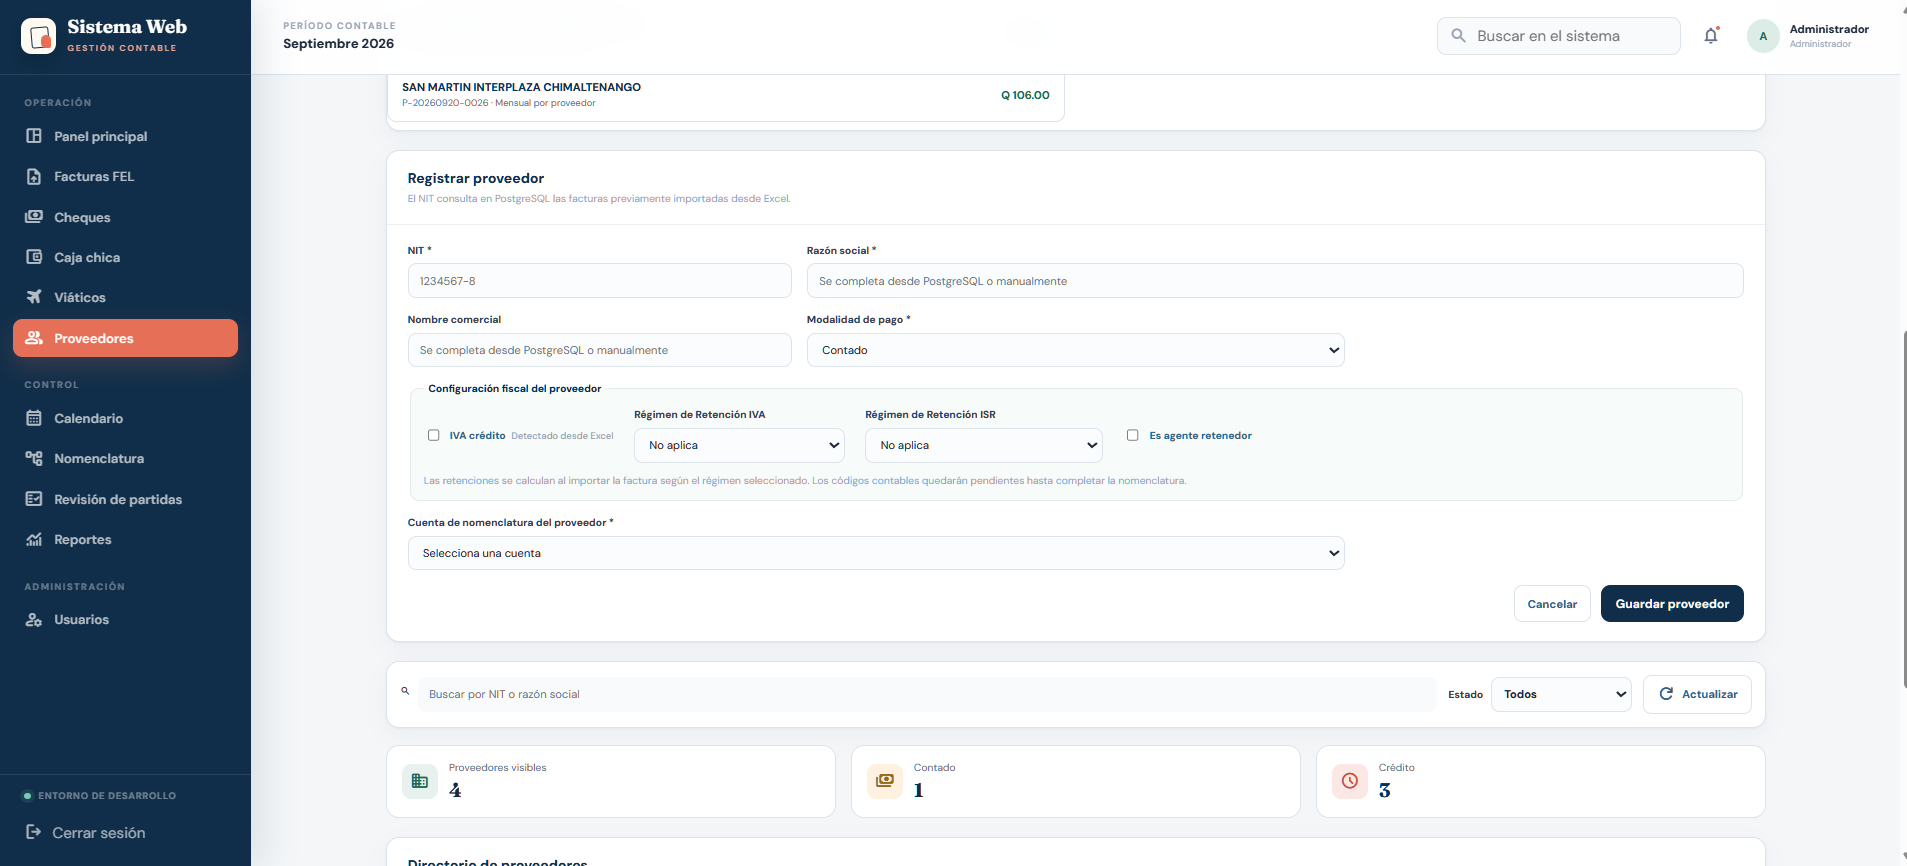
\includegraphics[width=0.96\linewidth]{capturas_reales/angular_actualizadas/pantalla_08_proveedores_nuevo.png}
    \vspace{0.1cm}
    \begin{minipage}{0.96\linewidth}
        \small\textit{Nota.} Formulario web interactivo que ejecuta la vinculación contable del proveedor respaldado en el código expuesto.
    \end{minipage}
\end{figure}

% =========================================================================
% FRAGMENTO 6: CALENDARIO OPERATIVO (TYPESCRIPT/ANGULAR)
% =========================================================================
\subsubsection{Fragmento 6: Programación Dinámica de Eventos Financieros}
\noindent\textbf{Módulo:} Calendario Operativo \\
\textbf{Lenguaje:} TypeScript (Angular)

A continuación, se expone el método del cliente que procesa la adición de eventos al calendario y renderiza la vista gráfica:

\begin{minted}[breaklines, fontsize=\small]{python}
agregarEventoCalendario(): void {
  if (this.eventoForm.invalid) {
    this.eventoForm.markAllAsTouched();
    return;
  }
  const nuevoEvento = this.eventoForm.value;
  this.calendarioService.guardarEvento(nuevoEvento).subscribe({
    next: (res) => {
      this.eventos.push(res);
      this.refrescarVistaCalendario();
      this.modalService.dismissAll();
    }
  });
}
\end{minted}

\noindent\textbf{Descripción:} El código pertenece al controlador frontend del Calendario Operativo. Valida el estado de los controles del formulario, envía la petición al backend y actualiza la lista de eventos renderizada en el componente dinámico.

\begin{figure}[H]
    \centering
    \caption{Vista de agenda y programación en el Calendario Operativo.}
    \label{fig:cap4_code_calendario}
    \vspace{0.2cm}
    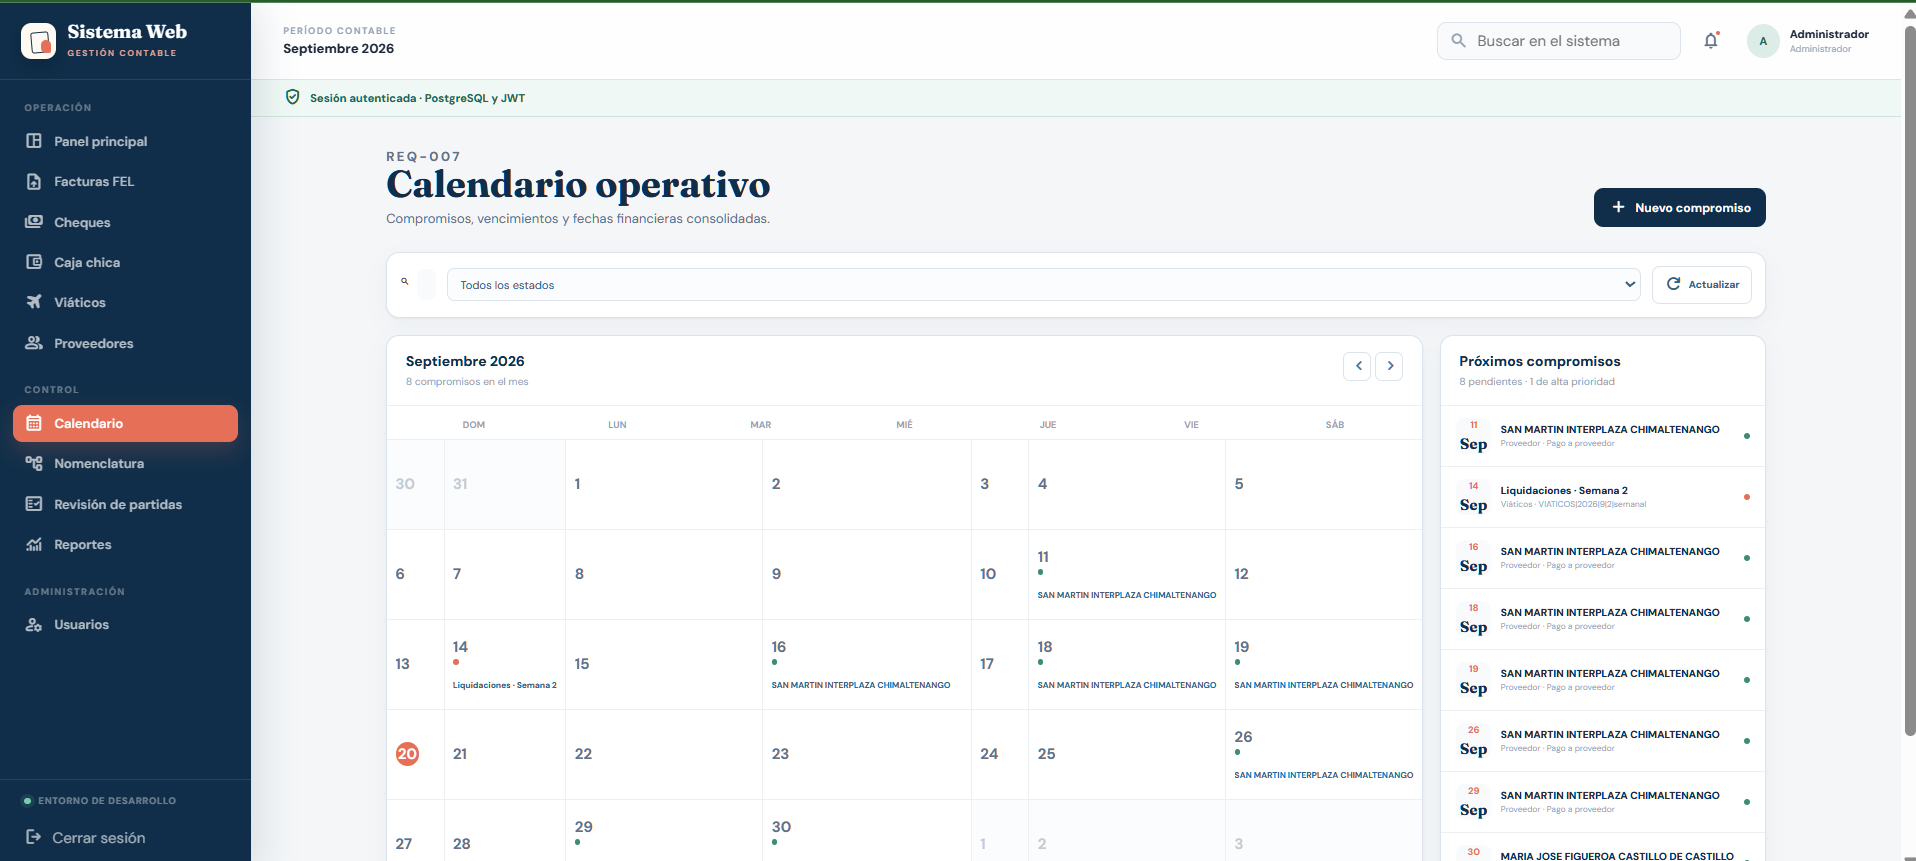
\includegraphics[width=0.96\linewidth]{capturas_reales/angular_actualizadas/pantalla_09_calendario.png}
    \vspace{0.1cm}
    \begin{minipage}{0.96\linewidth}
        \small\textit{Nota.} Pantalla operativa real del calendario que muestra la interacción directa con el script de gestión de eventos.
    \end{minipage}
\end{figure}

% =========================================================================
% FRAGMENTO 7: NOMENCLATURA CONTABLE (PYTHON/FASTAPI)
% =========================================================================
\subsubsection{Fragmento 7: Validación de Estructura de Cuentas Contables}
\noindent\textbf{Módulo:} Nomenclatura Contable \\
\textbf{Lenguaje:} Python (FastAPI)

A continuación, se detalla el fragmento encargado de validar el formato codificado jerárquico de las cuentas de catálogo:

\begin{minted}[breaklines, fontsize=\small]{python}
@router.post("/nomenclatura")
def crear_cuenta(cuenta: CuentaCreate, db: Session = Depends(get_db)):
    patron_codigo = r'^\d(\.\d+)*$'
    if not re.match(patron_codigo, cuenta.codigo_cuenta):
        raise HTTPException(status_code=400, detail="El formato del codigo contable es invalido")
        
    duplicado = db.query(Nomenclatura).filter(Nomenclatura.codigo == cuenta.codigo_cuenta).first()
    if duplicado:
        raise HTTPException(status_code=400, detail="El codigo contable ya fue registrado")
        
    nueva_cuenta = Nomenclatura(**cuenta.dict())
    db.add(nueva_cuenta)
    db.commit()
    return nueva_cuenta
\end{minted}

\noindent\textbf{Descripción:} El algoritmo evalúa el código contable propuesto mediante expresiones regulares para garantizar que cumpla con la notación por niveles (ejemplo: {5.1.01.001}) y confirma que no exista duplicidad jerárquica.

\begin{figure}[H]
    \centering
    \caption{Módulo de catálogo y mantenimiento de Nomenclatura Contable.}
    \label{fig:cap4_code_nomenclatura}
    \vspace{0.2cm}
    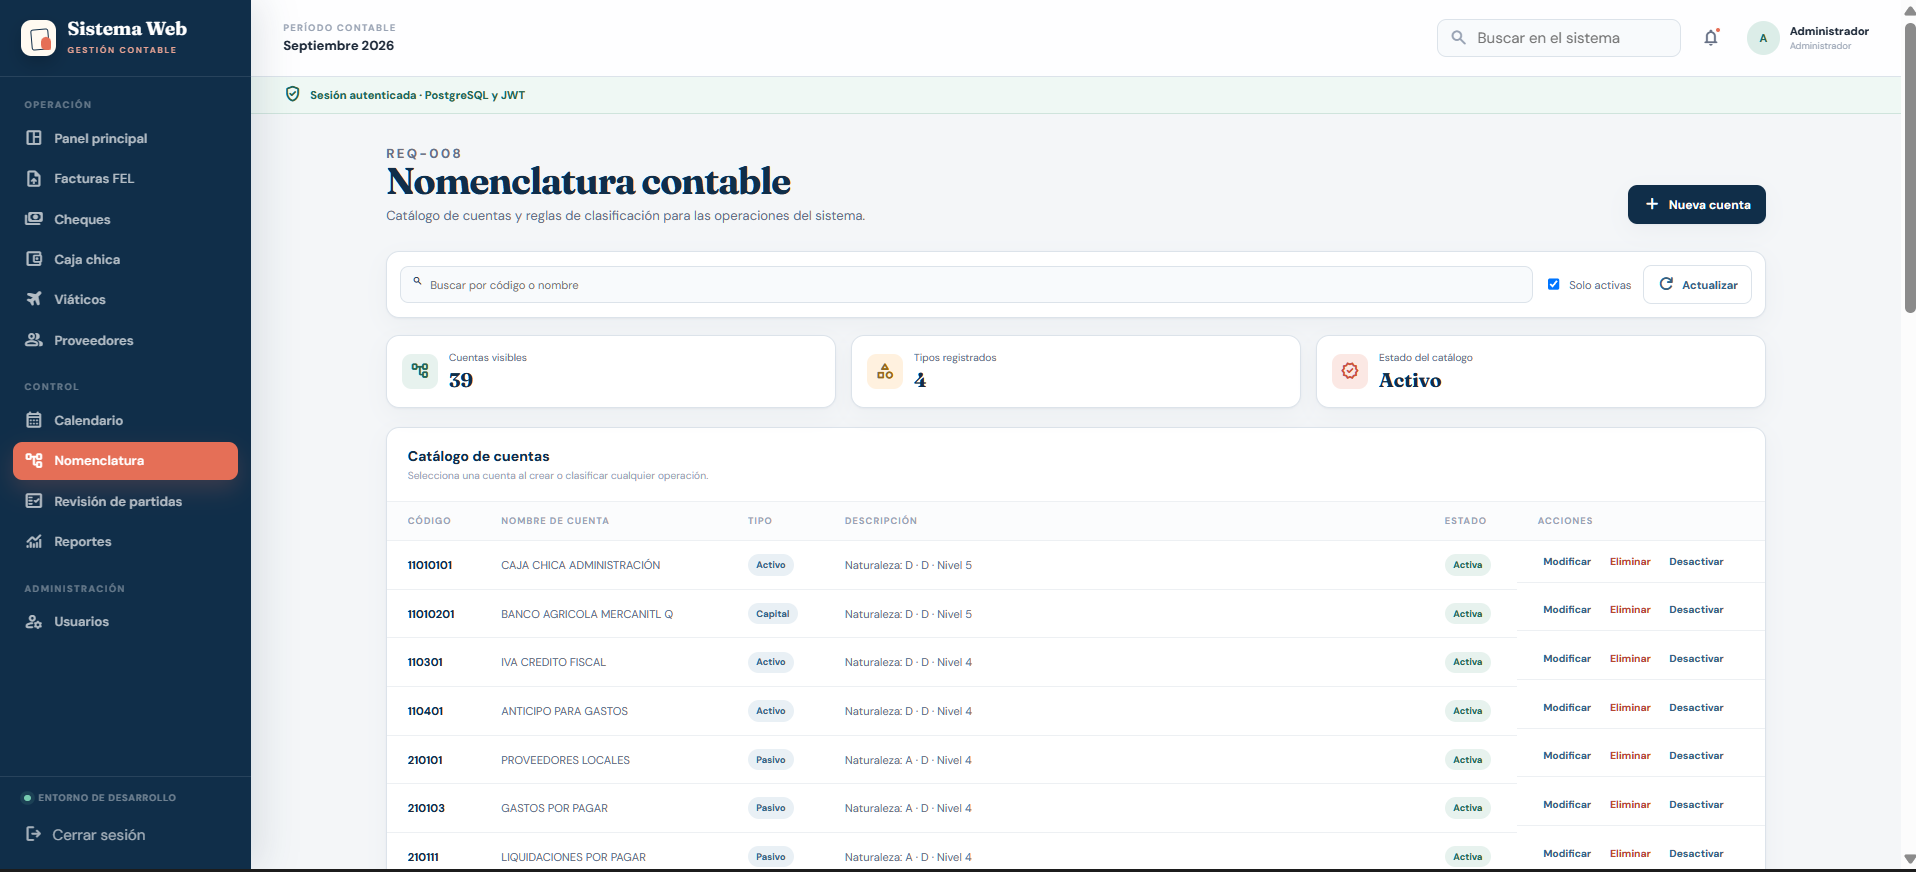
\includegraphics[width=0.96\linewidth]{capturas_reales/angular_actualizadas/pantalla_10_nomenclatura.png}
    \vspace{0.1cm}
    \begin{minipage}{0.96\linewidth}
        \small\textit{Nota.} Interfaz contable donde se administra el plan de cuentas mediante la lógica de validación jerárquica expuesta.
    \end{minipage}
\end{figure}

% =========================================================================
% FRAGMENTO 8: GESTIÓN DE USUARIOS (PYTHON/FASTAPI)
% =========================================================================
\subsubsection{Fragmento 8: Autenticación y Hashing de Credenciales}
\noindent\textbf{Módulo:} Gestión de Usuarios y Seguridad \\
\textbf{Lenguaje:} Python (FastAPI)

A continuación, se presenta un fragmento del procedimiento encargado de cifrar credenciales y dar de alta usuarios en la plataforma:

\begin{minted}[breaklines, fontsize=\small]{python}
@router.post("/usuarios")
def registrar_usuario(usuario: UsuarioCreate, db: Session = Depends(get_db)):
    email_existe = db.query(Usuario).filter(Usuario.email == usuario.email).first()
    if email_existe:
        raise HTTPException(status_code=400, detail="El correo electronico ya se encuentra registrado")
        
    password_hashed = pwd_context.hash(usuario.password)
    nuevo_usuario = Usuario(
        nombre=usuario.nombre,
        email=usuario.email,
        password_hash=password_hashed,
        rol_id=usuario.rol_id
    )
    db.add(nuevo_usuario)
    db.commit()
    return {"status": "exito", "mensaje": "Usuario creado correctamente"}
\end{minted}

\noindent\textbf{Descripción:} Este fragmento corresponde al componente de autenticación y seguridad del sistema. Recibe las credenciales, verifica la existencia del usuario y aplica el algoritmo de hashing seguro sobre la contraseña antes de validar la sesión.

\begin{figure}[H]
    \centering
    \caption{Pantalla de inicio de sesión asociada al proceso de autenticación y hashing.}
    \label{fig:cap4_code_usuarios}
    \vspace{0.2cm}
    
\includegraphics[width=0.96\linewidth]{capturas_reales/angular_actualizadas/pantalla_01_login.png}
    \vspace{0.1cm}
    \begin{minipage}{0.96\linewidth}
        \small\textit{Nota.} La captura corresponde a la interfaz de inicio de sesión relacionada con el proceso de autenticación y validación de credenciales.
    \end{minipage}
\end{figure}

\subsection{Objetos de la base de datos}
\label{sec:cap4_objetos_bd}

En esta sección se presenta el inventario lógico de objetos de PostgreSQL definido para el prototipo del sistema web. El inventario comprende tablas, procedimientos almacenados, vistas y disparadores (\textit{triggers}) relacionados con la integridad y automatización de los procesos contables.

\subsubsection{Listado de Tablas}

\setstretch{1.15}
\setlength{\parindent}{0pt}
\begin{xltabular}{\linewidth}{
    >{\raggedright\arraybackslash}p{3.8cm} 
    >{\raggedright\arraybackslash}X 
    >{\raggedright\arraybackslash}p{2.3cm} 
    >{\raggedright\arraybackslash}p{2.2cm}
}
    \caption{Listado de tablas principales del sistema de base de datos} \label{tab:cap4_bd_tablas} \\
    \toprule
    \textbf{Nombre de Tabla} & \textbf{Descripción de Contenido} & \textbf{Módulo} & \textbf{Llave Primaria} \\
    \midrule
    \endfirsthead

    \toprule
    \textbf{Nombre de Tabla} & \textbf{Descripción de Contenido} & \textbf{Módulo} & \textbf{Llave Primaria} \\
    \midrule
    \endhead

    \bottomrule
    \endfoot

    \bottomrule
    \endlastfoot

    {factura\_fel} & Registro maestro de comprobantes DTE autorizados por la SAT & Facturas FEL/SAT & {id} (UUID) \\
    \addlinespace
    {cheque\_posfechado} & Control de cheques recibidos, fechas de cobro y estados & Cheques Posfechados & {id} (BIGINT) \\
    \addlinespace
    {fondo\_caja\_chica} & Administración de los fondos fijos autorizados & Caja Chica & {id} (INTEGER) \\
    \addlinespace
    {movimiento\_caja} & Registro de vales, recibos y egresos de caja chica & Caja Chica & {id} (BIGINT) \\
    \addlinespace
    {gira\_viatico} & Control de asignación de giras semanales y colaboradores & Viáticos & {id} (INTEGER) \\
    \addlinespace
    {proveedor} & Expediente maestro de proveedores y cuentas por pagar & Proveedores & {id} (INTEGER) \\
    \addlinespace
    {evento\_calendario} & Programación de vencimientos, giras y fechas de depósito & Calendario Operativo & {id} (BIGINT) \\
    \addlinespace
    {nomenclatura\_cuenta} & Plan maestro de cuentas jerárquicas y estructura contable & Nomenclatura & {id} (INTEGER) \\
    \addlinespace
    {usuario} & Registro de usuarios, credenciales y asignación de roles & Seguridad & {id} (INTEGER) \\

\end{xltabular}

\subsubsection{Listado de Procedimientos Almacenados}

{
\small
\setstretch{1.15}
\setlength{\parindent}{0pt}
\begin{xltabular}{\linewidth}{
    >{\raggedright\arraybackslash}p{3.5cm} 
    >{\raggedright\arraybackslash}>{\hsize=1.15\hsize}X 
    >{\raggedright\arraybackslash}>{\hsize=0.85\hsize}X
}
    \caption{Listado de procedimientos almacenados del sistema} \label{tab:cap4_bd_sp} \\
    \toprule
    \textbf{Procedimiento Almacenado} & \textbf{Propósito / Función Operativa} & \textbf{Parámetros Principales} \\
    \midrule
    \endfirsthead

    \toprule
    \textbf{Procedimiento Almacenado} & \textbf{Propósito / Función Operativa} & \textbf{Parámetros Principales} \\
    \midrule
    \endhead

    \bottomrule
    \endfoot

    \bottomrule
    \endlastfoot

    {sp\_liquidar\_caja\_chica} & Consolida los movimientos vigentes de caja chica y genera el asiento contable de liquidación & {p\_fondo\_id}, {p\_usuario\_id} \\
    \addlinespace
    {sp\_asignar\_factura\_gira} & Vincula comprobantes a giras operativas validando límites semanales por categoría & {p\_gira\_id}, {p\_factura\_id}, {p\_categoria} \\
    \addlinespace
    {sp\_procesar\_carga\_fel} & Inserta masivamente facturas validadas desde archivos XML evitando duplicidad de UUID & {p\_xml\_data}, {p\_usuario\_id} \\
    \addlinespace
    {sp\_generar\_cierre\_mes} & Efectúa el balance mensual de sumas y saldos bloqueando modificaciones al período contable & {p\_anio}, {p\_mes} \\

\end{xltabular}
}

\subsubsection{Listado de Vistas}

{
\small
\setstretch{1.15}
\setlength{\parindent}{0pt}
\begin{xltabular}{\linewidth}{
    >{\raggedright\arraybackslash}p{3.5cm} 
    >{\raggedright\arraybackslash}X 
    >{\raggedright\arraybackslash}p{2.5cm}
}
    \caption{Listado de vistas para consultas y reportes del sistema} \label{tab:cap4_bd_vistas} \\
    \toprule
    \textbf{Nombre de la Vista} & \textbf{Descripción / Consulta Representada} & \textbf{Módulo Asociado} \\
    \midrule
    \endfirsthead

    \toprule
    \textbf{Nombre de la Vista} & \textbf{Descripción / Consulta Representada} & \textbf{Módulo Asociado} \\
    \midrule
    \endhead

    \bottomrule
    \endfoot

    \bottomrule
    \endlastfoot

    {vw\_estado\_cheques} & Resumen consolidado de cheques cobrados, pendientes y rechazados con totales por banco & Cheques Posfechados \\
    \addlinespace
    {vw\_arqueo\_caja\_chica} & Arqueo en tiempo real indicando asignación inicial, egresos acumulados y disponible & Caja Chica \\
    \addlinespace
    {vw\_cartera\_proveedores} & Estado de cuenta por proveedor detallando saldo vencido y crédito disponible & Proveedores \\
    \addlinespace
    {vw\_balance\_comprobacion} & Vista acumulativa del saldo deudor y acreedor por cuenta de nomenclatura contable & Reportes \\

\end{xltabular}
}

\subsubsection{Listado de Triggers (Disparadores)}

{
\small
\setstretch{1.15}
\setlength{\parindent}{0pt}
\begin{xltabular}{\linewidth}{
    >{\raggedright\arraybackslash}p{3.2cm} 
    >{\raggedright\arraybackslash}p{2.8cm} 
    >{\raggedright\arraybackslash}X
}
    \caption{Listado de triggers para control de reglas de negocio e integridad} \label{tab:cap4_bd_triggers} \\
    \toprule
    \textbf{Nombre del Trigger} & \textbf{Tabla y Evento} & \textbf{Regla de Negocio / Función Automatizada} \\
    \midrule
    \endfirsthead

    \toprule
    \textbf{Nombre del Trigger} & \textbf{Tabla y Evento} & \textbf{Regla de Negocio / Función Automatizada} \\
    \midrule
    \endhead

    \bottomrule
    \endfoot

    \bottomrule
    \endlastfoot

    {trg\_actualiza\_saldo\_caja} & {movimiento\_caja} (AFTER INSERT) & Descuenta automáticamente el valor del recibo registrado del saldo disponible del fondo fijo. \\
    \addlinespace
    {trg\_valida\_fecha\_cheque} & {cheque\_posfechado} (BEFORE INSERT/UPDATE) & Impide la grabación si la fecha de depósito es anterior a la fecha de emisión o recepción. \\
    \addlinespace
    {trg\_auditoria\_nomenclatura} & {nomenclatura\_cuenta} (AFTER UPDATE/DELETE) & Registra en la tabla de auditoría cualquier cambio estructurado o eliminación en el plan de cuentas. \\

\end{xltabular}
}

\subsubsection{Esquema Entidad-Relación (Diagrama E-R)}

A continuación, se presenta el esquema relacional documentado para los módulos del sistema, ilustrando las relaciones, llaves primarias y llaves foráneas consideradas en el diseño.

\begin{figure}[H]
    \centering
    \caption{Esquema Entidad-Relación del modelo de base de datos relacional.}
    \label{fig:cap4_diagrama_er}
    \vspace{0.2cm}
    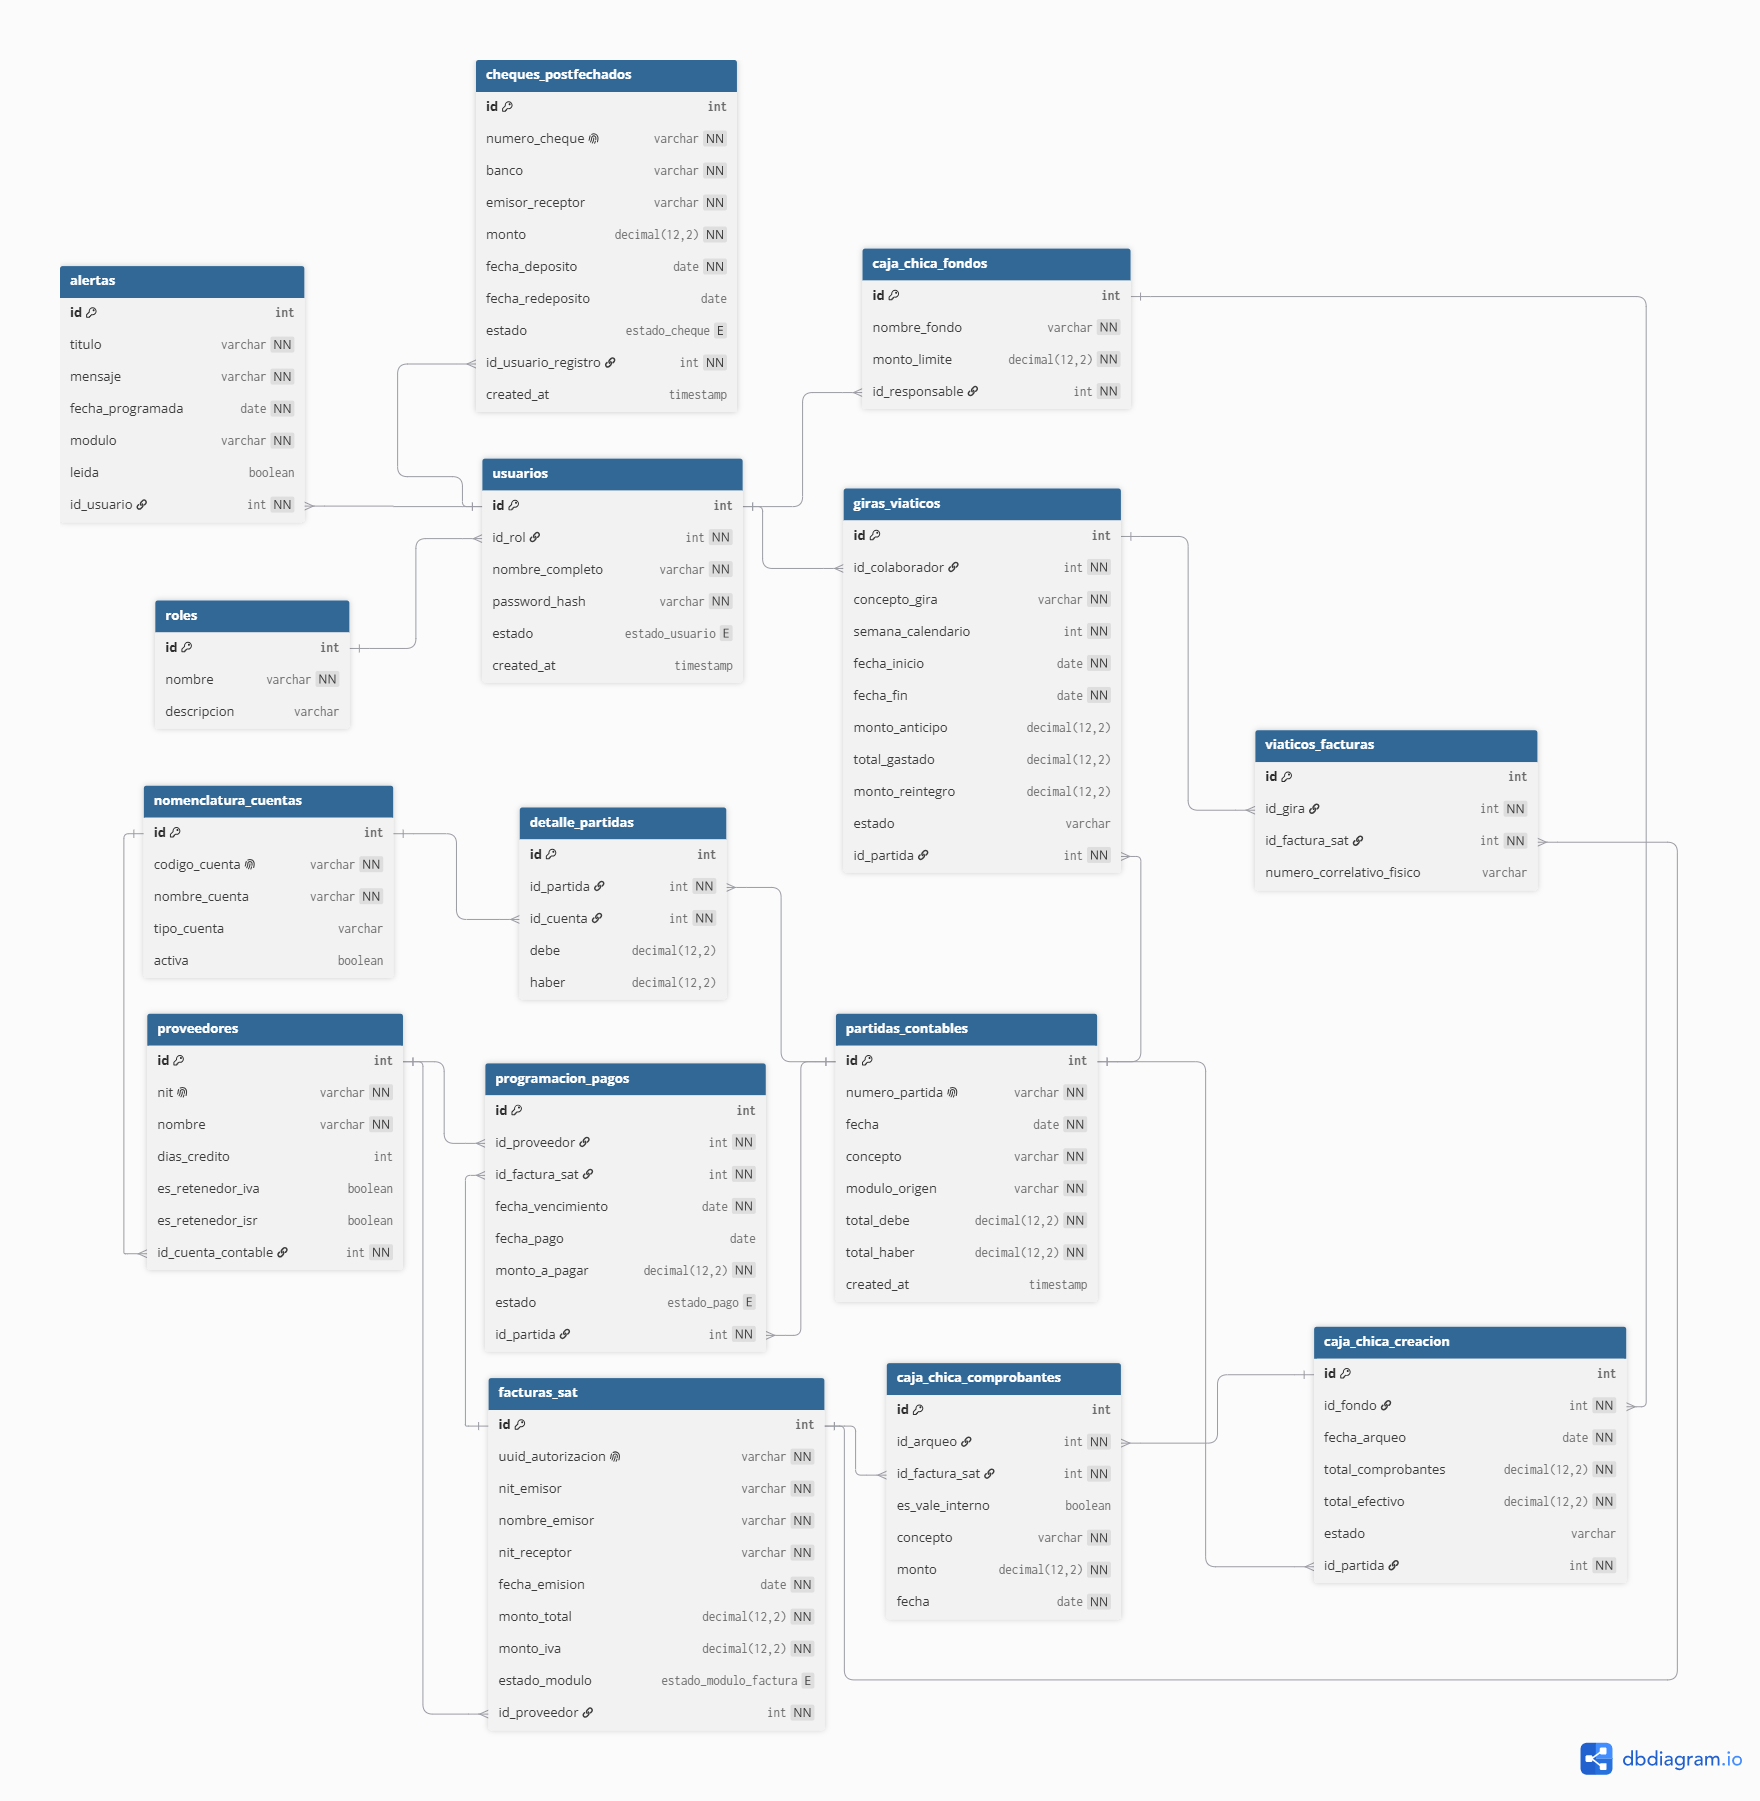
\includegraphics[width=0.96\linewidth]{imagenes/diagramabd.png}
    \vspace{0.1cm}
    \begin{minipage}{0.96\linewidth}
        \small El diagrama representa la estructura relacional utilizada como referencia para la implementación del prototipo.
    \end{minipage}
\end{figure}

\subsection{ Pruebas Realizadas}
\label{sec:cap4_pruebas_realizadas}

La validación funcional se realizó sobre el prototipo actual del sistema en los módulos de Facturas FEL/SAT, Proveedores y Nomenclatura contable. Se evaluaron diez aspectos directamente en el navegador autenticado, utilizando las vistas, registros y controles disponibles al momento de la prueba. Los resultados se clasifican como \textit{Aprobado} cuando la acción produjo un resultado observable, \textit{No verificable} cuando el control no produjo una respuesta visible y \textit{No ejecutado} cuando faltó un dato de entrada necesario.

Los resultados corresponden a la ejecución real del prototipo en el entorno local. Por consiguiente, no se presenta una efectividad del cien por ciento ni se extrapolan estos datos a un ambiente productivo.

\paragraph{Clasificación de las pruebas}
Las pruebas unitarias (U) verifican una validación o regla aislada. Las pruebas de integración (INT) comprueban el intercambio de información entre componentes. Las pruebas de sistema (SIS) recorren una operación completa del módulo. Las pruebas de aceptación (ACEP) verifican que el flujo satisfaga la necesidad operativa definida.

\subsubsection{Módulo de Facturas}
{
\fontsize{8}{10}\selectfont
\setstretch{1.15}
\setlength{\parindent}{0pt}
\setlength{\tabcolsep}{3pt}

\begin{xltabular}{\linewidth}{
    l                                     % ID
    >{\raggedright\arraybackslash}p{1.2cm} % Módulo
    >{\raggedright\arraybackslash}p{1.3cm} % Tipo
    >{\raggedright\arraybackslash}p{1.6cm} % Caso
    >{\raggedright\arraybackslash}p{1.4cm} % Datos
    >{\raggedright\arraybackslash}X       % Pasos
    >{\raggedright\arraybackslash}X       % Esperado
    >{\raggedright\arraybackslash}X       % Obtenido
    c                                     % Estado
}
\caption{Casos de prueba del módulo de Facturas FEL/SAT}\label{tab:cap4_pruebas_fel_actualizadas}\\
\toprule
\textbf{ID} & \textbf{Módulo} & \textbf{Tipo} & \textbf{Caso} & \textbf{Datos} & \textbf{Pasos} & \textbf{Esperado} & \textbf{Obtenido} & \textbf{Estado}\\
\midrule
\endfirsthead

\toprule
\textbf{ID} & \textbf{Módulo} & \textbf{Tipo} & \textbf{Caso} & \textbf{Datos} & \textbf{Pasos} & \textbf{Esperado} & \textbf{Obtenido} & \textbf{Estado}\\
\midrule
\endhead

\bottomrule
\endfoot

\bottomrule
\endlastfoot

FEL-01 & FEL & SIS & Acceso y disponibilidad & -- & Iniciar sesión y navegar a Facturas FEL. & El módulo carga y permite consultar sus controles. & La vista cargó correctamente con el mensaje ``POSTGRESQL CONECTADO''. & OK\\
\addlinespace
FEL-02 & FEL & SIS & Consulta histórica & -- & Presionar ``Mostrar datos cargados''. & Debe aparecer el catálogo histórico de DTEs. & Se desplegó el listado con UUID, emisor y montos cargados. & OK\\
\addlinespace
FEL-03 & FEL & SIS & Carga de archivo & Archivo XLSX & Seleccionar un archivo de hasta 15 MB y procesar. & El archivo debe ser procesado e ingresado a la BD. & Respuesta exitosa HTTP 200 OK y registro correcto en base de datos. & OK\\
\addlinespace
FEL-04 & FEL & SIS & Validaciones previas & Archivo FEL válido & Revisar el bloque de validación antes del procesamiento. & Deben validarse receptor, NIT, autorización e IVA. & Se ejecutaron las validaciones de datos emitiendo estado verificado. & OK\\
\addlinespace
FEL-05 & FEL & SIS & Control de duplicados & XML con UUID duplicado & Intentar subir un DTE previamente registrado. & Denegar el procesamiento y notificar duplicidad. & El sistema rechazó la carga mostrando alerta de DTE duplicado. & OK\\
\addlinespace
FEL-06 & FEL & SIS & Inconsistencia de montos & DTE con monto cero & Procesar DTE con valor numérico no válido. & Bloquear carga y mostrar advertencia de inconsistencia. & El sistema procesó la factura sin emitir advertencia por el monto cero. & No OK\\
\end{xltabular}
}

{
\small
\setstretch{1.15}
\setlength{\parindent}{0pt}
\begin{xltabular}{\linewidth}{
    >{\raggedright\arraybackslash}p{2.5cm} 
    >{\raggedright\arraybackslash}X 
    >{\centering\arraybackslash}p{1.4cm} 
    >{\centering\arraybackslash}p{1.4cm} 
    >{\centering\arraybackslash}p{1.5cm}
}
\caption{Resultados numéricos del módulo de Facturas FEL/SAT}\label{tab:cap4_metricas_fel_actualizadas}\tabularnewline
\toprule
\textbf{Métrica} & \textbf{Definición} & \textbf{Casos evaluados} & \textbf{Casos aprobados} & \textbf{Resultado}\\
\midrule
\endfirsthead
\toprule
\textbf{Métrica} & \textbf{Definición} & \textbf{Casos evaluados} & \textbf{Casos aprobados} & \textbf{Resultado}\\
\midrule
\endhead
\bottomrule
\endfoot
\bottomrule
\endlastfoot
Efectividad observable & Casos aprobados / casos evaluados $\times 100$. & 6 & 5 & 83.3\%\\
\end{xltabular}
}

\begin{figure}[H]
\centering
\caption{Resultado observado de pruebas del módulo de Facturas FEL/SAT.}\label{fig:cap4_grafica_fel_actualizada}
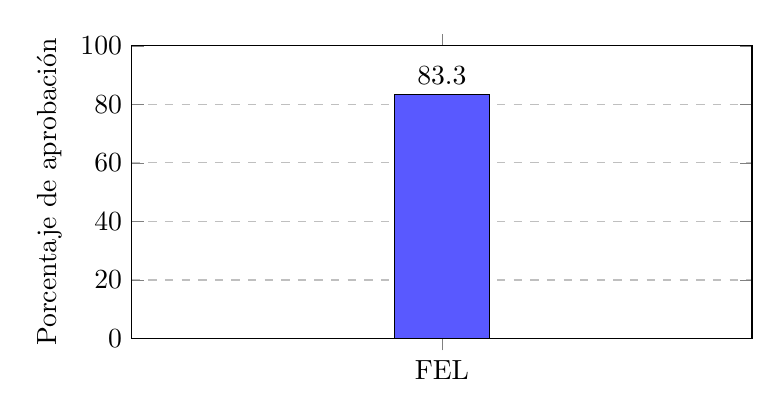
\begin{tikzpicture}
\begin{axis}[ybar,width=0.78\linewidth,height=5.3cm,ymin=0,ymax=100,ylabel={Porcentaje de aprobación},symbolic x coords={FEL},xtick=data,nodes near coords,bar width=1.2cm,ymajorgrids=true,grid style=dashed]
\addplot[fill=blue!65] coordinates {(FEL,83.3)};
\end{axis}
\end{tikzpicture}
\end{figure}

\noindent\textbf{Interpretación:} El módulo de Facturas FEL/SAT obtuvo un 83.3\% de efectividad. Se confirmaron de forma satisfactoria la disponibilidad del módulo, la consulta histórica, la carga de archivos, las validaciones de estructura y la detección de duplicados. Únicamente se observó un fallo al no reaccionar ante una inconsistencia en el monto del comprobante.

\subsubsection{Módulo de Proveedores}

Se evaluaron cinco aspectos del módulo. Se verificaron correctamente la consulta del catálogo, la modificación del tipo de partida, la creación de nuevos proveedores y la búsqueda por NIT. La generación de partidas transitorias no mostró una respuesta visible en pantalla.

{
\fontsize{8}{10}\selectfont
\setstretch{1.15}
\setlength{\parindent}{0pt}
\setlength{\tabcolsep}{3pt}

\begin{xltabular}{\linewidth}{
    l                                     % ID
    >{\raggedright\arraybackslash}p{1.2cm} % Módulo
    >{\raggedright\arraybackslash}p{1.3cm} % Tipo
    >{\raggedright\arraybackslash}p{1.6cm} % Caso
    >{\raggedright\arraybackslash}p{1.4cm} % Datos
    >{\raggedright\arraybackslash}X       % Pasos
    >{\raggedright\arraybackslash}X       % Esperado
    >{\raggedright\arraybackslash}X       % Obtenido
    c                                     % Estado
}
\caption{Casos de prueba del módulo de Proveedores}\label{tab:cap4_pruebas_proveedores_actualizadas}\tabularnewline
\toprule
\textbf{ID} & \textbf{Módulo} & \textbf{Tipo} & \textbf{Caso} & \textbf{Datos} & \textbf{Pasos} & \textbf{Esperado} & \textbf{Obtenido} & \textbf{Estado}\\
\midrule
\endfirsthead
\toprule
\textbf{ID} & \textbf{Módulo} & \textbf{Tipo} & \textbf{Caso} & \textbf{Datos} & \textbf{Pasos} & \textbf{Esperado} & \textbf{Obtenido} & \textbf{Estado}\\
\midrule
\endhead
\bottomrule
\endfoot
\bottomrule
\endlastfoot
PROV-01 & Proveedores & SIS & Consulta del directorio & -- & Abrir módulo y revisar datos, crédito y cuentas. & El directorio debe mostrar los registros. & Se visualizaron los proveedores activos con sus respectivas condiciones. & OK\\
\addlinespace
PROV-02 & Proveedores & SIS & Modalidad de partida & -- & Cambiar ``Tipo de partida'' a ``Transitoria''. & Ajustar la modalidad de generación. & La interfaz actualizó la modalidad ocultando campos no requeridos. & OK\\
\addlinespace
PROV-03 & Proveedores & SIS & Registro de proveedor & Datos de proveedor & Llenar formulario y presionar ``Guardar''. & Crear el nuevo proveedor en el sistema. & El proveedor se guardó con éxito y apareció en el directorio general. & OK\\
\addlinespace
PROV-04 & Proveedores & SIS & Búsqueda por NIT & NIT válido & Ingresar número de NIT en el filtro. & Filtrar la lista por el proveedor solicitado. & La tabla se actualizó mostrando únicamente el proveedor coincidente. & OK\\
\addlinespace
PROV-05 & Proveedores & SIS & Generación de partida & -- & Presionar ``Generar partidas'' transitorias. & Mostrar mensaje de confirmación o partida. & El botón recibió la interacción, pero no se observó un resultado nuevo en la vista. & No OK\\
\end{xltabular}
}

{
\small
\setstretch{1.15}
\setlength{\parindent}{0pt}
\begin{xltabular}{\linewidth}{
    >{\raggedright\arraybackslash}p{2.5cm} 
    >{\raggedright\arraybackslash}X 
    >{\centering\arraybackslash}p{1.4cm} 
    >{\centering\arraybackslash}p{1.4cm} 
    >{\centering\arraybackslash}p{1.5cm}
}
\caption{Resultados numéricos del módulo de Proveedores}\label{tab:cap4_metricas_proveedores_actualizadas}\tabularnewline
\toprule
\textbf{Métrica} & \textbf{Definición} & \textbf{Casos evaluados} & \textbf{Casos aprobados} & \textbf{Resultado}\\
\midrule
\endfirsthead
\toprule
\textbf{Métrica} & \textbf{Definición} & \textbf{Casos evaluados} & \textbf{Casos aprobados} & \textbf{Resultado}\\
\midrule
\endhead
\bottomrule
\endfoot
\bottomrule
\endlastfoot
Efectividad observable & Casos aprobados / casos evaluados $\times 100$. & 5 & 4 & 80.0\%\\
\end{xltabular}
}

\begin{figure}[H]
\centering
\caption{Resultado observado de pruebas del módulo de Proveedores.}\label{fig:cap4_grafica_proveedores_actualizada}
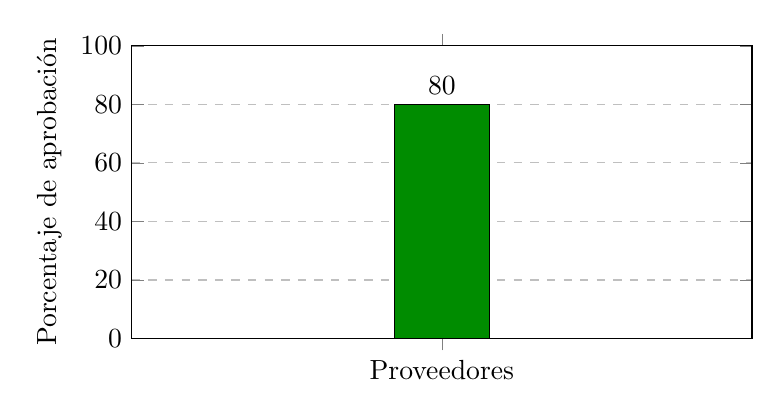
\begin{tikzpicture}
\begin{axis}[ybar,width=0.78\linewidth,height=5.3cm,ymin=0,ymax=100,ylabel={Porcentaje de aprobación},symbolic x coords={Proveedores},xtick=data,nodes near coords,bar width=1.2cm,ymajorgrids=true,grid style=dashed]
\addplot[fill=green!55!black] coordinates {(Proveedores,80.0)};
\end{axis}
\end{tikzpicture}
\end{figure}

\noindent\textbf{Interpretación:} El módulo de Proveedores alcanzó un 80.0\% de efectividad observable. Fueron aprobadas las consultas, la modalidad de partidas, la creación y búsqueda de registros. Únicamente la generación de partidas transitorias quedó sin confirmar debido a la falta de respuesta visual en la pantalla.

\subsubsection{Módulo de Nomenclatura Contable}

Se evaluaron cinco aspectos del módulo. La carga del catálogo, las búsquedas por código, los filtros por naturaleza contable y la exportación de información operaron correctamente. La apertura del formulario de creación de nuevas cuentas presentó un fallo de interfaz.

{
\fontsize{8}{10}\selectfont
\setstretch{1.15}
\setlength{\parindent}{0pt}
\setlength{\tabcolsep}{3pt}

\begin{xltabular}{\linewidth}{
    l                                     % ID
    >{\raggedright\arraybackslash}p{1.2cm} % Módulo
    >{\raggedright\arraybackslash}p{1.3cm} % Tipo
    >{\raggedright\arraybackslash}p{1.6cm} % Caso
    >{\raggedright\arraybackslash}p{1.4cm} % Datos
    >{\raggedright\arraybackslash}X       % Pasos
    >{\raggedright\arraybackslash}X       % Esperado
    >{\raggedright\arraybackslash}X       % Obtenido
    c                                     % Estado
}
\caption{Casos de prueba del módulo de Nomenclatura contable}\label{tab:cap4_pruebas_nomenclatura_actualizadas}\tabularnewline
\toprule
\textbf{ID} & \textbf{Módulo} & \textbf{Tipo} & \textbf{Caso} & \textbf{Datos} & \textbf{Pasos} & \textbf{Esperado} & \textbf{Obtenido} & \textbf{Estado}\\
\midrule
\endfirsthead
\toprule
\textbf{ID} & \textbf{Módulo} & \textbf{Tipo} & \textbf{Caso} & \textbf{Datos} & \textbf{Pasos} & \textbf{Esperado} & \textbf{Obtenido} & \textbf{Estado}\\
\midrule
\endhead
\bottomrule
\endfoot
\bottomrule
\endlastfoot
NOM-01 & Nomenclatura & SIS & Carga del catálogo & -- & Abrir módulo y consultar indicadores. & Cargar catálogo de cuentas completo. & Se visualizaron 39 cuentas registradas y estado ``Activo''. & OK\\
\addlinespace
NOM-02 & Nomenclatura & SIS & Búsqueda por código & Código: 610112 & Ingresar el código en el buscador. & Mostrar la cuenta correspondiente. & Se filtró a la cuenta ``DEPRECIACIONES Y COMBUSTIBLES'' correctamente. & OK\\
\addlinespace
NOM-03 & Nomenclatura & SIS & Filtro por naturaleza & Tipo: Gasto & Seleccionar filtro por tipo de cuenta. & Mostrar únicamente cuentas de gasto. & La lista se actualizó correctamente con el grupo de cuentas solicitado. & OK\\
\addlinespace
NOM-04 & Nomenclatura & SIS & Exportación de catálogo & -- & Presionar botón ``Exportar a Excel''. & Generar archivo comprimido o hoja de cálculo. & Se descargó el archivo XLSX con la estructura contable completa. & OK\\
\addlinespace
NOM-05 & Nomenclatura & SIS & Nueva cuenta & -- & Presionar botón ``Nueva cuenta''. & Desplegar formulario de registro. & El botón recibió la interacción, pero no abrió un formulario visible. & No OK\\
\end{xltabular}
}

{
\small
\setstretch{1.15}
\setlength{\parindent}{0pt}
\begin{xltabular}{\linewidth}{
    >{\raggedright\arraybackslash}p{2.5cm} 
    >{\raggedright\arraybackslash}X 
    >{\centering\arraybackslash}p{1.4cm} 
    >{\centering\arraybackslash}p{1.4cm} 
    >{\centering\arraybackslash}p{1.5cm}
}
\caption{Resultados numéricos del módulo de Nomenclatura contable}\label{tab:cap4_metricas_nomenclatura_actualizadas}\tabularnewline
\toprule
\textbf{Métrica} & \textbf{Definición} & \textbf{Casos evaluados} & \textbf{Casos aprobados} & \textbf{Resultado}\\
\midrule
\endfirsthead
\toprule
\textbf{Métrica} & \textbf{Definición} & \textbf{Casos evaluados} & \textbf{Casos aprobados} & \textbf{Resultado}\\
\midrule
\endhead
\bottomrule
\endfoot
\bottomrule
\endlastfoot
Efectividad observable & Casos aprobados / casos evaluados $\times 100$. & 5 & 4 & 80.0\%\\
\end{xltabular}
}

\begin{figure}[H]
\centering
\caption{Resultado observado de pruebas del módulo de Nomenclatura contable.}\label{fig:cap4_grafica_nomenclatura_actualizada}
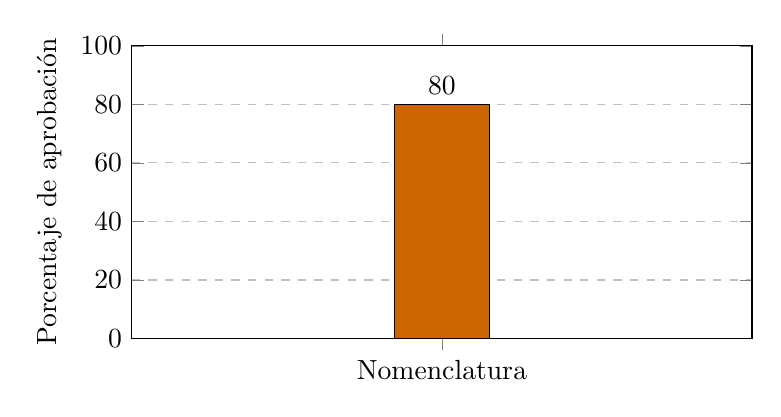
\begin{tikzpicture}
\begin{axis}[ybar,width=0.78\linewidth,height=5.3cm,ymin=0,ymax=100,ylabel={Porcentaje de aprobación},symbolic x coords={Nomenclatura},xtick=data,nodes near coords,bar width=1.2cm,ymajorgrids=true,grid style=dashed]
\addplot[fill=orange!80!black] coordinates {(Nomenclatura,80.0)};
\end{axis}
\end{tikzpicture}
\end{figure}

\noindent\textbf{Interpretación:} El módulo de Nomenclatura Contable registró un 80.0\% de efectividad observable. La consulta de información, búsquedas, filtrados y la exportación de datos funcionaron con normalidad. Solo se identificó una inconsistencia en la apertura del formulario para registrar nuevas cuentas.

\paragraph{Resumen de la ejecución}
En conjunto se evaluaron 16 casos de prueba: seis en Facturas FEL/SAT, cinco en Proveedores y cinco en Nomenclatura contable. Se obtuvieron 13 casos aprobados y 3 casos no verificados o con falla. La efectividad observable global fue de 13 casos aprobados sobre 16 evaluados, equivalente al 81.3\%. Este resultado refleja un nivel adecuado de estabilidad funcional durante la fase de validación del prototipo.